
% to choose your degree
% please un-comment just one of the following
\documentclass[bsc,frontabs,twoside,singlespacing,parskip,deptreport]{infthesis}     % for BSc, BEng etc.
% \documentclass[minf,frontabs,twoside,singlespacing,parskip,deptreport]{infthesis}  % for MInf
\usepackage{todonotes}
\usepackage{hyperref}
\usepackage{minted}

\begin{document}


\title{CoStor, a distributed backup solution}

\author{Robert Phipps}

\course{Computer Science}
\project{4th Year Project Report}

\date{\today}

\abstract{
CoStor is a proof of concept cloud backup solution, making use of simple to manage 
HTTPS requests for all communication and synchronisation across the system, allowing for 
easy integration into existing environments. Authentication is managed by tokens and
role-based authorisation, with configuration for the client set with an easily deployable
YAML file.\newline

This implementation makes use of two primary components, a command line client application,
which builds a database of and fingerprints the directory tree to be backed up, and a Django
based server application, which is used as the sync endpoint for offsite storage of backup
data. These communicate using the HTTP API to identify file binaries and metadata that need
to be transferred, and a multi-stage, resumable upload process is used to upload
large files to the system.\newline

It uses generic objects and datastructure fingerprints to allow server-side deduplication of
backed up data across clients, and allows backup "snapshots" to be restored as archives from
the web UI of the server application.
}

\maketitle

\section*{Acknowledgements}

This project makes extensive use of concepts and architectures explored in this paper from
Paul Anderson and Le Zhang: Fast and secure laptop backups with encrypted de-duplication
\cite{macbac-lisa}

Many thanks to Paul Anderson for his supervision of this project.

\tableofcontents

\pagenumbering{arabic}


\chapter{Solution overview}

CoStor is designed as a turnkey solution to the problem of maintaining reliable system
backups within an SME with multiple sites, such as a confederation of schools. Instead
of using expensive and bandwidth intensive cloud storage services for offsite backup, 
CoStor is designed to hold a complete local backup on-site within the CoStor server, as
well as automatically replicating backup data across a group of federated instances of
the server software, ensuring that there is always at least two redundant copies of the
backup datastore in two different physical locations.

To simplify networking requirements for deployment, all communication between clients 
and servers, both locally and between sites, makes use of standard HTTPS requests. This 
negates the need for complex multi-site VPNs, and simply requires a single TCP port to
be forwarded to the server from the internet.

The backup datastore's metadata and directory structures are maintained inside an SQL
database and can only be modified over the HTTP API, reducing attack surface
compared to making use of more traditional file transfer methods like FTP, NFS or 
SSHFS.

All management is completed through a simple web UI, where agents can be added, 
authentication tokens can be created and the backup history subsequently monitored. 
Users can browse the directory trees for each backup "snapshot" in the event that a file 
needs to be recovered. A full backup restore can be completed by requesting a restoration 
archive, whereby the server will build a complete archive of a snapshot, pulling data from its
local datastore, or from other sites in the event of a remote restore\footnote{Remote restore 
has not been fully implemented}.

This system makes use of Django for server-side components, a Python web framework with
fantastic ORM and enforcement of best-practices. The client side database is managed with
PonyORM, running on top of SQLite.

\clearpage

\section{Goals of CoStor}

Given the target organisations for CoStor, there are some specific goals that need to be 
targeted during development.

\begin{itemize}
	\item \textbf{Reliable backups}
		\subitem As should be very obvious, being a backup solution, CoStor needs to be
		able to reliably manage and maintain backups for a network. This includes
		protections such as an "append-only" API for backup clients, validation of 
		uploaded data, and mitigations against the most common reasons a backup
		may be called upon such as accidental deletion, user errors, hardware failure and 
		ransomware style attacks.
	\item \textbf{Simple restores}
		\subitem As this system is targeted at small organisations which may not have their
		own full-time IT support staff, restoring from backups should be straightforward 
		for an end-user. This is achieved through the use of a self-service web UI.
	\item \textbf{Robust security and audit logs}
		\subitem Backups almost always contain confidential information, so CoStor needs 
		to be able to manage permissions on a granular user-by-user basis. It also needs 
		to include audit logging for all operations on the system. Any offsite storage and
		"data in flight" needs to be strongly encrypted to protect confidentiality.
	\item \textbf{Low maintenance}
		\subitem Systems tend to be forgotten about, and in the case of backups, often you
		only notice something hasn't been working once you need to restore 
		something\footnote{GitLab found this to their cost in 2017 after discovering their 
		backups hadn't been running for some time: 
		\url{https://techcrunch.com/2017/02/01/gitlab-suffers-major-backup-failure-after-data-deletion-incident/}},
		so CoStor needs to automatically maintain its database and include robust database 
		integrity checking to ensure that the system is ready when the user needs it most.
	\item \textbf{Simple deployment}
		\subitem Again, CoStor needs to be deployable by inexperienced IT support staff
		without prior knowledge of network filesystems, command line interfaces or web
		development. This can be achieved by making use of clever packaging and deployment 
		strategies such as Docker for server components and zero-touch installation scripts
		for backup clients. By making use of standard and well understood protocols such
		as HTTP(S) for communication between components, compatibility with most network
		architectures should be maintained, without the requirement for complex network 
		share configurations, multi-site VPNs and authentication systems.
	\item \textbf{Centralised management and monitoring}
		\subitem As this is designed to be deployed over a large number of client PCs,
		ensuring configuration is correct could be challenging. As such, CoStor will allow 
		setup to be pushed to clients using a simple config file. Backup
		logs will also be maintained on the server so that an administrator can monitor their
		entire estate from a single place.
	\item \textbf{Distributed and fault-tolerant file stores}
		\subitem Leaving the best to last, CoStor's standout feature will be that backups
		can be automatically replicated between federated instances of the CoStor server, 
		over a zero-configuration HTTPS link. The system should be able to recover from the
		loss of a server without any data loss, and allow restoration of data originating
		from any site from any of the remaining instances of CoStor within the network.
		\subitem \textit{(Unfortunately, distributed backup was not able to be implemented
		ahead of the deadline for this project.)}
\end{itemize}

\section{Limitation of scope for the purposes of this project}

This project was proposed as a two-year task, as part of the MInf course. Due to circumstance
changes, this project has been condensed into a single year as part of the BSci. This has 
required many of the user interface elements and advanced features to be removed from scope.

As such, in its current state, CoStor is a single-server solution, which would require a 
traditional second tier of redundancy for the backup store, such as scheduled \texttt{rsync}
tasks to a remote filestore, or hardware redundant storage including LTO tape archives. 
Support for these is not included in the CoStor proof of concept provided here. The methodology
and structure of a potential cross-site replication implementation is however included in this 
report, as it offers context to a number of design decisions. As data currently does not leave
the corporate network, backups are not encrypted at rest, and only with standard HTTP TLS in 
flight. There is no need to restrict access to specific systems' backups as the CoStor 
administrator will already have access to all users' documents as a network administrator.

The management of local filesystem metadata was considerably more challenging than the timescale
for this project anticipated, with the CoStor client requiring far more logic within it than was
intended. This resulted in available time for the server application to be limited.

\clearpage

\section{Exploration of existing solutions}

There are many packages in existence which incorporate a subset of the features targeted
by this project, however most either focus on the synchronisation features with some 
limited support for file history, and no robust backup capability, whereas others rely on
cloud storage infrastructure as the backend, distributed datastore which either necessitates
the use of a commercial provider such as AWS S3\footnote{Amazon Web Services' bucket 
storage solution} or BackBlaze B2. Both of these greatly increase cost and introduce a 
reliance on a third party.

\subsection{Overviews}

A number of existing products have been selected as they offer the closest functionality
to that targeted by CoStor. Here we take a high-level look at featuresets and methodologies
used by these solutions:

\subsubsection{Syncthing}

Syncthing is a service targeted at consumers who want a self-hosted alternative to commercial
cloud storage and synchronisation services such as Dropbox, Google Drive and OneDrive. The 
agent software can be configured to sync any file changes between two or more devices, allowing
for access anywhere, with a form of georeplication. It also requires fairly minimal network
configuration, just needing a pair of ports to be opened on at least one of the nodes to allow
discovery of other agents.

A very large distinction has to be made in the fact that "Syncthing is a continuous file 
synchronization program"\cite{syncthing}, in that it isn't designed to create restorable 
snapshots of your data, and therefore is completely unsuitable for robust \textit{backup} of 
important information.

More information is available at \url{https://syncthing.net} \cite{syncthing}

\subsubsection{UrBackup}

UrBackup is closer to CoStor in its goals, as is specifically built to be used as a backup 
system. It can auto-discover agents on the network, and begin incremental backups to its server
software. It also supports full image backups of NTFS formatted drives with bare metal 
restore. UrBackup has many of the features targeted by CoStor, including a simple web interface
for management, however it does not include any built-in support for georeplication.

More information is available at \url{https://www.urbackup.org/index.html} \cite{urbackup}

\subsubsection{Hermes}

Hermes is an "open-source redundant distributed storage network"\cite{hermes}. Although it
doesn't come pre-packaged with components allowing it to be used as a turnkey backup system,
it is worth exploring as it does specifically target the geo-replication features for the 
purposes of backup that CoStor is looking to integrate. It promises fast, encrypted and seamless
replication and sharding of data across nodes in the network, making use of LZMA compression
to increase performance.

This would appear to be a very promising option to integrate as the backend storage for CoStor,
however it looks like the project is very much stale, with the last commits being made in late 
2014. As such, its codebase is somewhat limited in utility, given its lack of ongoing 
maintenance. It is also written in Go, with limited documentation, which is not a language
that I am familiar enough with to begin work on reviving.

More information is available at \url{https://github.com/Hermes/hermes} \cite{hermes}

\subsubsection{Bacula}

Bacula is an open-source and very mature backup framework, with tools to allow a multitude of
network configurations. Unfortunately its flexibilty does result in the software being complex
to configure. CoStor is targeting small organisations with limited in-house IT support capacity,
so this would likely be too complex to deploy without the assistance of external contractors. 
Bacula is also available in an "enterprise" edition\cite{bacula-ent}, which includes 
support as part of the subscription cost, however this version is both closed-source and
not inconsiderably expensive.

More information is available at \url{https://www.bacula.org} \cite{bacula}

\subsubsection{Amanda}

Amanda is another backup-specific solution, again with a "community edition" being accompanied
by a commercially supported "enterprise" version of the software. Like the other systems 
investigated, it targets backup to local storage, NAS drives and traditional tape backup
libraries, so would not be suitable for the use case targeted by CoStor.

More information is available at \url{https://www.zmanda.com/amanda-community-edition.html} \cite{zmanda}

\subsubsection{GlusterFS}

The Gluster filesystem is a "software scalable network filesystem"\cite{gluster-home}, which 
allows systems administrators to build complex filesystems across multiple physical machines
using commodity hardware. Gluster is targeted at engineers designing private cloud environments
which need large volumes of storage accessible from many devices, and has a huge number of 
configuration options to allow, among other things, redundant replicated storage across machines.
It also has support for filesystem filters that can offer encryption at a filesystem level before
data is transmitted between nodes.

Unfortunately for CoStor's usecase, this system is built on the assumption that the Gluster 
volumes are configured at the point of deployment, by the same user on all sites. It also is
primarily managed through a command line interface, with limited Python bindings, and is targeted
at an architecture where all nodes have rights to see data within the volume. Finally, it is
based around a master-slave architecture, which is unsuitable if CoStor were to be using a shared
volume for all nodes. It would be possible to wrangle a Gluster configuration to match what is
required by CoStor, where each site has its own volume, with its own georeplication session, 
however this would be very difficult to automatically provision from the CoStor web interface, 
and should be mostly unnecessary given the data structure used for backups.

More information is available at \url{https://www.gluster.org} \cite{gluster-home}

\subsection{Case study: Git}

Git is one of the most well known versioning and distributed storage systems, and works in a very
similar way to how CoStor is intended to behave. It maintains a local database of all file data, 
storing file history within the records for each file. It supports delta-replication to one or
many local or offsite Git servers, with the ability to recover data from any point on time that
has been "committed" to the history.

\subsubsection{Data storage}

The Pro Git Second Edition documentation \cite{progit} states that "Git is a content-addressable filesystem. [...]
What this means that at the core of Git is a simple key-value data store."

Everything in Git is stored as generic objects, with their SHA-1 hash making up their unique ID
within the datastore. These can be data objects, tree objects and commit objects, all interlinked by
ID to form a representation of the versioned filesystem. These objects are stored as files within
the \texttt{.git/} subdirectory created when Git is initialised. (Figure \ref{fig:gitfs})

\begin{figure}
	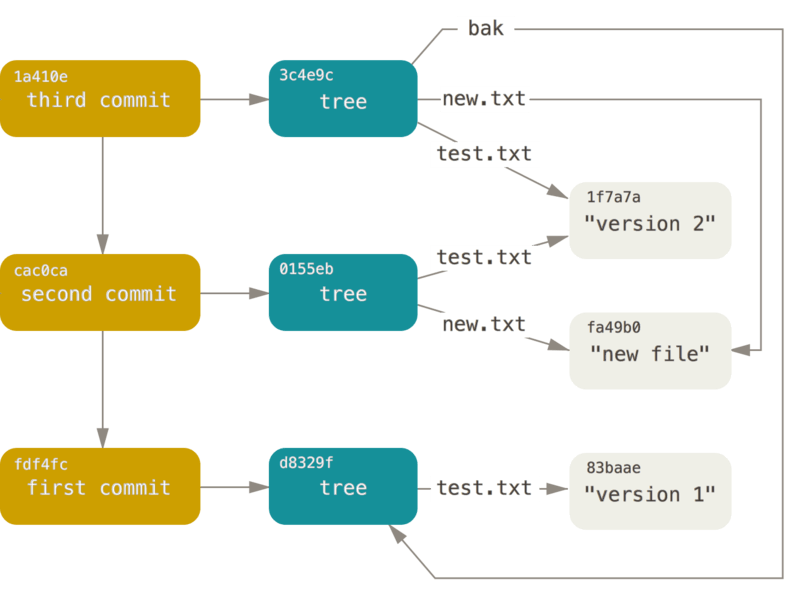
\includegraphics[width=0.6\paperwidth]{img/git-tree}
	\caption{Representation of the Git content addressable filesystem \cite{progit}}
	\label{fig:gitfs}
\end{figure}

All directory structure and file metadata is stored in the tree object for a commit, with file data
being stored in a separate 'blob' object and referenced by the tree. This allows a single copy 
of the file to be used as the "backup" copy for multiple commits without requiring multiple
copies of the file to be stored, reducing disk usage considerably as most commits only touch a few
of the files within the repository.

Git also selectively processes file metadata, for example only including the three UNIX file modes for
normal files, symlinks and executable files. This simplifies processing and makes behaviour 
predictable for the end user. It also mitigates any chance of accidentally interacting with special
devices such as serial ports and pipes, which could confuse the system.

Occasionally, the client creates delta compressed "packfiles" of the objects, explained later.

\subsubsection{Data transfer}

For data transfer, Git can use either an SSH based protocol, which they call "The Smart Protocol",
or a "Dumb" HTTP based protocol. For the purposes of CoStor, this HTTP based protocol is of more
relevance, as we are trying to avoid reliance on "exotic"\footnote{Yes, SSH isn't exactly exotic, but port 22 is commonly blocked on company firewalls, along with networks that use an HTTP proxy for web filtering and monitoring} 
protocols.

First, the client makes a GET request to pull down the SHA-1 IDs of the branch that the user
is interested in, or in Git terminology, the client requests the HEAD reference. Once it has
that reference, it is able to make a further request to the specific commit required, by its
SHA-1 ID. The commit contains a reference to its tree object, and the parent commit, which gives
the client everything it needs to rebuild the entire commit history. Some data can be bundled into
packfiles, in which case the Git server will simply HTTP 404 and the client will have to make a 
few more requests to work out the packfile containing the commit.

For making commits, the client first builds packfiles, which is where it takes all of the objects and 
performs delta compression to reduce the transfer size. It looks for files that are named and sized 
similarly before trying to calculate the difference between the files. This can drastically save on 
space compared to uploading the "loose" data objects. And, as these packfiles contain an entire 
copy of the Git datastore, this can be uploaded as one file to the server.

\subsubsection{Evaluation}

This is a very elegant solution to the problem, and allows Git to be a very simple and portable
version control system. However, its reliance on a standard filesystem for the datastore does
potentially make management of that data more complex, as there is no support for foreign key 
relationships or the ability to make use of an ORM to ensure the database integrity is maintained.

In the case of Git, there is normally at least one other copy of the database, so if it is 
corrupted on the local machine, it can be rebuilt from that copy.

The generalised data structure of generic "objects", representing everything the system needs to
keep track of, however could be very easily replicated within an ORM. Storing the binary data
separately from the file metadata can also enable us to deduplicate files across systems, with 
not only multiple trees from the same repository sharing a blob database, but multiple trees from
multiple systems running the backup client software and sharing the same server instance.

An important thing to note, is that there appears to be no use of filesystem snapshots: Git
relies on files not being written to or changed while it indexes the repository. This means it
would not be suitable for backing up live application datastores or constantly changing data
such as web server databases unless the database server application is shut down while the 
commit is made.

\section{Deployment topology}

The basic topology of a CoStor network would be as follows:

\begin{itemize}
	\item \textbf{Clients} (many):
	\subitem The CoStor client software is installed on any systems which are to be backed up.
	It communicates over the local network to the site's local instance of the CoStor server.
	
	\item \textbf{Servers} (one per site/network):
	\subitem  There should be one instance of CoStor server on the internal private network of 
	any site that has clients to be backed up. There could be multiple instances running in one
	local network space, but they would operate as separate "sites" within the software. The 
	servers are the primary file store for a site, and manage replication between federated
	instances on other sites.
	
	\item \textbf{Federated servers} ($>2$ across multiple locations):
	\subitem These are additional instances of the server application, and can be on separate
	networks and in different physical locations. These communicate over the internet through
	a replication API to keep a redundant copy of all data from all servers. They can restore
	data from any site within the group in the event that a site's server fails, assuming the 
	target site's encryption key is provided.
\end{itemize}

\todo[inline]{TODO: Insert diagram of topology, and describe how data is distributed across the 
members of the CoStor network.}

\section{Specimen use case}

The initial inspiration for this project was a use case within a confederation of small, state
controlled schools. Each school currently spends a large amount of money on a third-party 
managed cloud backup solution - in the region of \pounds500 per year for only 20GB of backed
up data. This meant that they were unable to backup considerable portions of their data, leaving
some of their media based teaching resources vulnerable.

The purpose of the confederation is to allow the members to share resources and purchasing power
for resources that can be beneficial to all of them.

CoStor could be utilised by these schools to allow them to geo-replicate their backups among 
themselves, on commodity server hardware, allowing them to no longer be reliant on expensive
cloud backup solutions. Each site would have a single CoStor server appliance with their file
servers, databases, Microsoft Active Directory databases and any other critical data being
backed up by instances of CoStor client, allowing backups to complete rapidly across the high
speed LAN, with replication to other schools' CoStor servers being carried out overnight when 
the internet connection is quiet.

The system should be as close to turnkey and zero-maintenance as possible, allowing it to be
set up by their IT support contractors, and left to work for years at a time without much
interference.

\subsection{Revised use case}

To accommodate for the limits that have been applied to the scope of the project, the current
implementation is based off the following use case:

CoStor could be used by a small organisation, which requires a central backup for specific
directory sub-trees on networked workstations. The CoStor client is deployed along with a
config file to these systems, and scheduled with \texttt{cron} to run out of hours, when the
systems are not in use. These back up to the shared CoStor server, which deduplicates the
binary data of stored files to reduce disk usage when identical files are backed up from
multiple systems.

The server application would be managed through a web UI by the server administrator, and any
backup archives can be downloaded through this interface by them for any agents they manage.

\chapter{Client implementation}

\section{Summary}

CoStor clients are designed to be managed centrally through the CoStor server web interface,
therefore they require no GUI of their own, just a way to set the target server instance, 
required directory tree to backup (the backup root) and their authentication token. These are
set using a \texttt{.YAML} file, which is easy to push to clients with standard network 
management tools such as Microsoft Group Policy and Logon Scripts.

The client is built around Python 3, and PonyORM working in parallel with an SQlite database. 
This means there are very few dependencies, once the Python project is bundled, and allows
cross-platform development with a shared codebase.

The current client has been developed and tested on MacOS version 10.15 Catalina with an APFS
filesystem. Porting file metadata processing to other filesystems is a non-trivial task, due 
to differences in the representations of this information. APFS is very similar to UNIX 
filesystems such as ext4, so should be compatible, however this is untested.

\section{The backup process}

The backup process works as follows:

\begin{enumerate}
	\item \textbf{Build directory structure hashes}:
	The client uses the \texttt{HashTreeMaker} class to build a simplified version of the 
	directory tree being backed up, traversing through the tree bottom-up, and building objects
	for every item it encounters, each item identified by a hash based off of its attributes
	and the hashes of all its children. File data is also hashed and stored with a path to the
	file, to be used for backup later.
	
	\item \textbf{Local metadata database update}:
	The client keeps a local database of all backup "snapshots" as trees of objects, created by
	the hasher. It checks for an existing snapshot, and uses this to identify any subtrees within
	the backup root which have changed since the last backup run. It then writes any changes to
	the database as part of a new snapshot.
	
	\item \textbf{Authenticate with server}:
	A quick test is made to ensure that the client's credentials are valid and that the server is
	accessible.
	
	\item \textbf{Create snapshot definitions}:
	Entries are created on the server to represent the backup "snaphot" within the database, and
	assigned to the agent.
	
	\item \textbf{Push changed metadata objects}:
	The server is queried to see if it has seen any objects with matching IDs (hashes), and any
	objects that are missing are pushed as a single JSON object. The IDs of unchanged objects
	that are used in this new snapshot are also pushed so they can be attached to the snapshot.
	
	\item \textbf{File "primes" are pushed to the server}:
	Again, the server is queried to check for existing copies of any of the files that are 
	included in this backup snapshot, by hash. For any files that are missing, the client uses
	the path included with the object to find a copy of that file, and pushes it to the server,
	in multiple chunks.
\end{enumerate}

\section{Large file upload API}

To allow large files to be uploaded over standard HTTPS connections, with the ability to recover
from connection issues, files are split into (currently 100MB) chunks, which are individually
hashed, and then pushed in sequence to the server. This process is detailed in Figure \ref{fig:lfileupload}.

\begin{figure}
	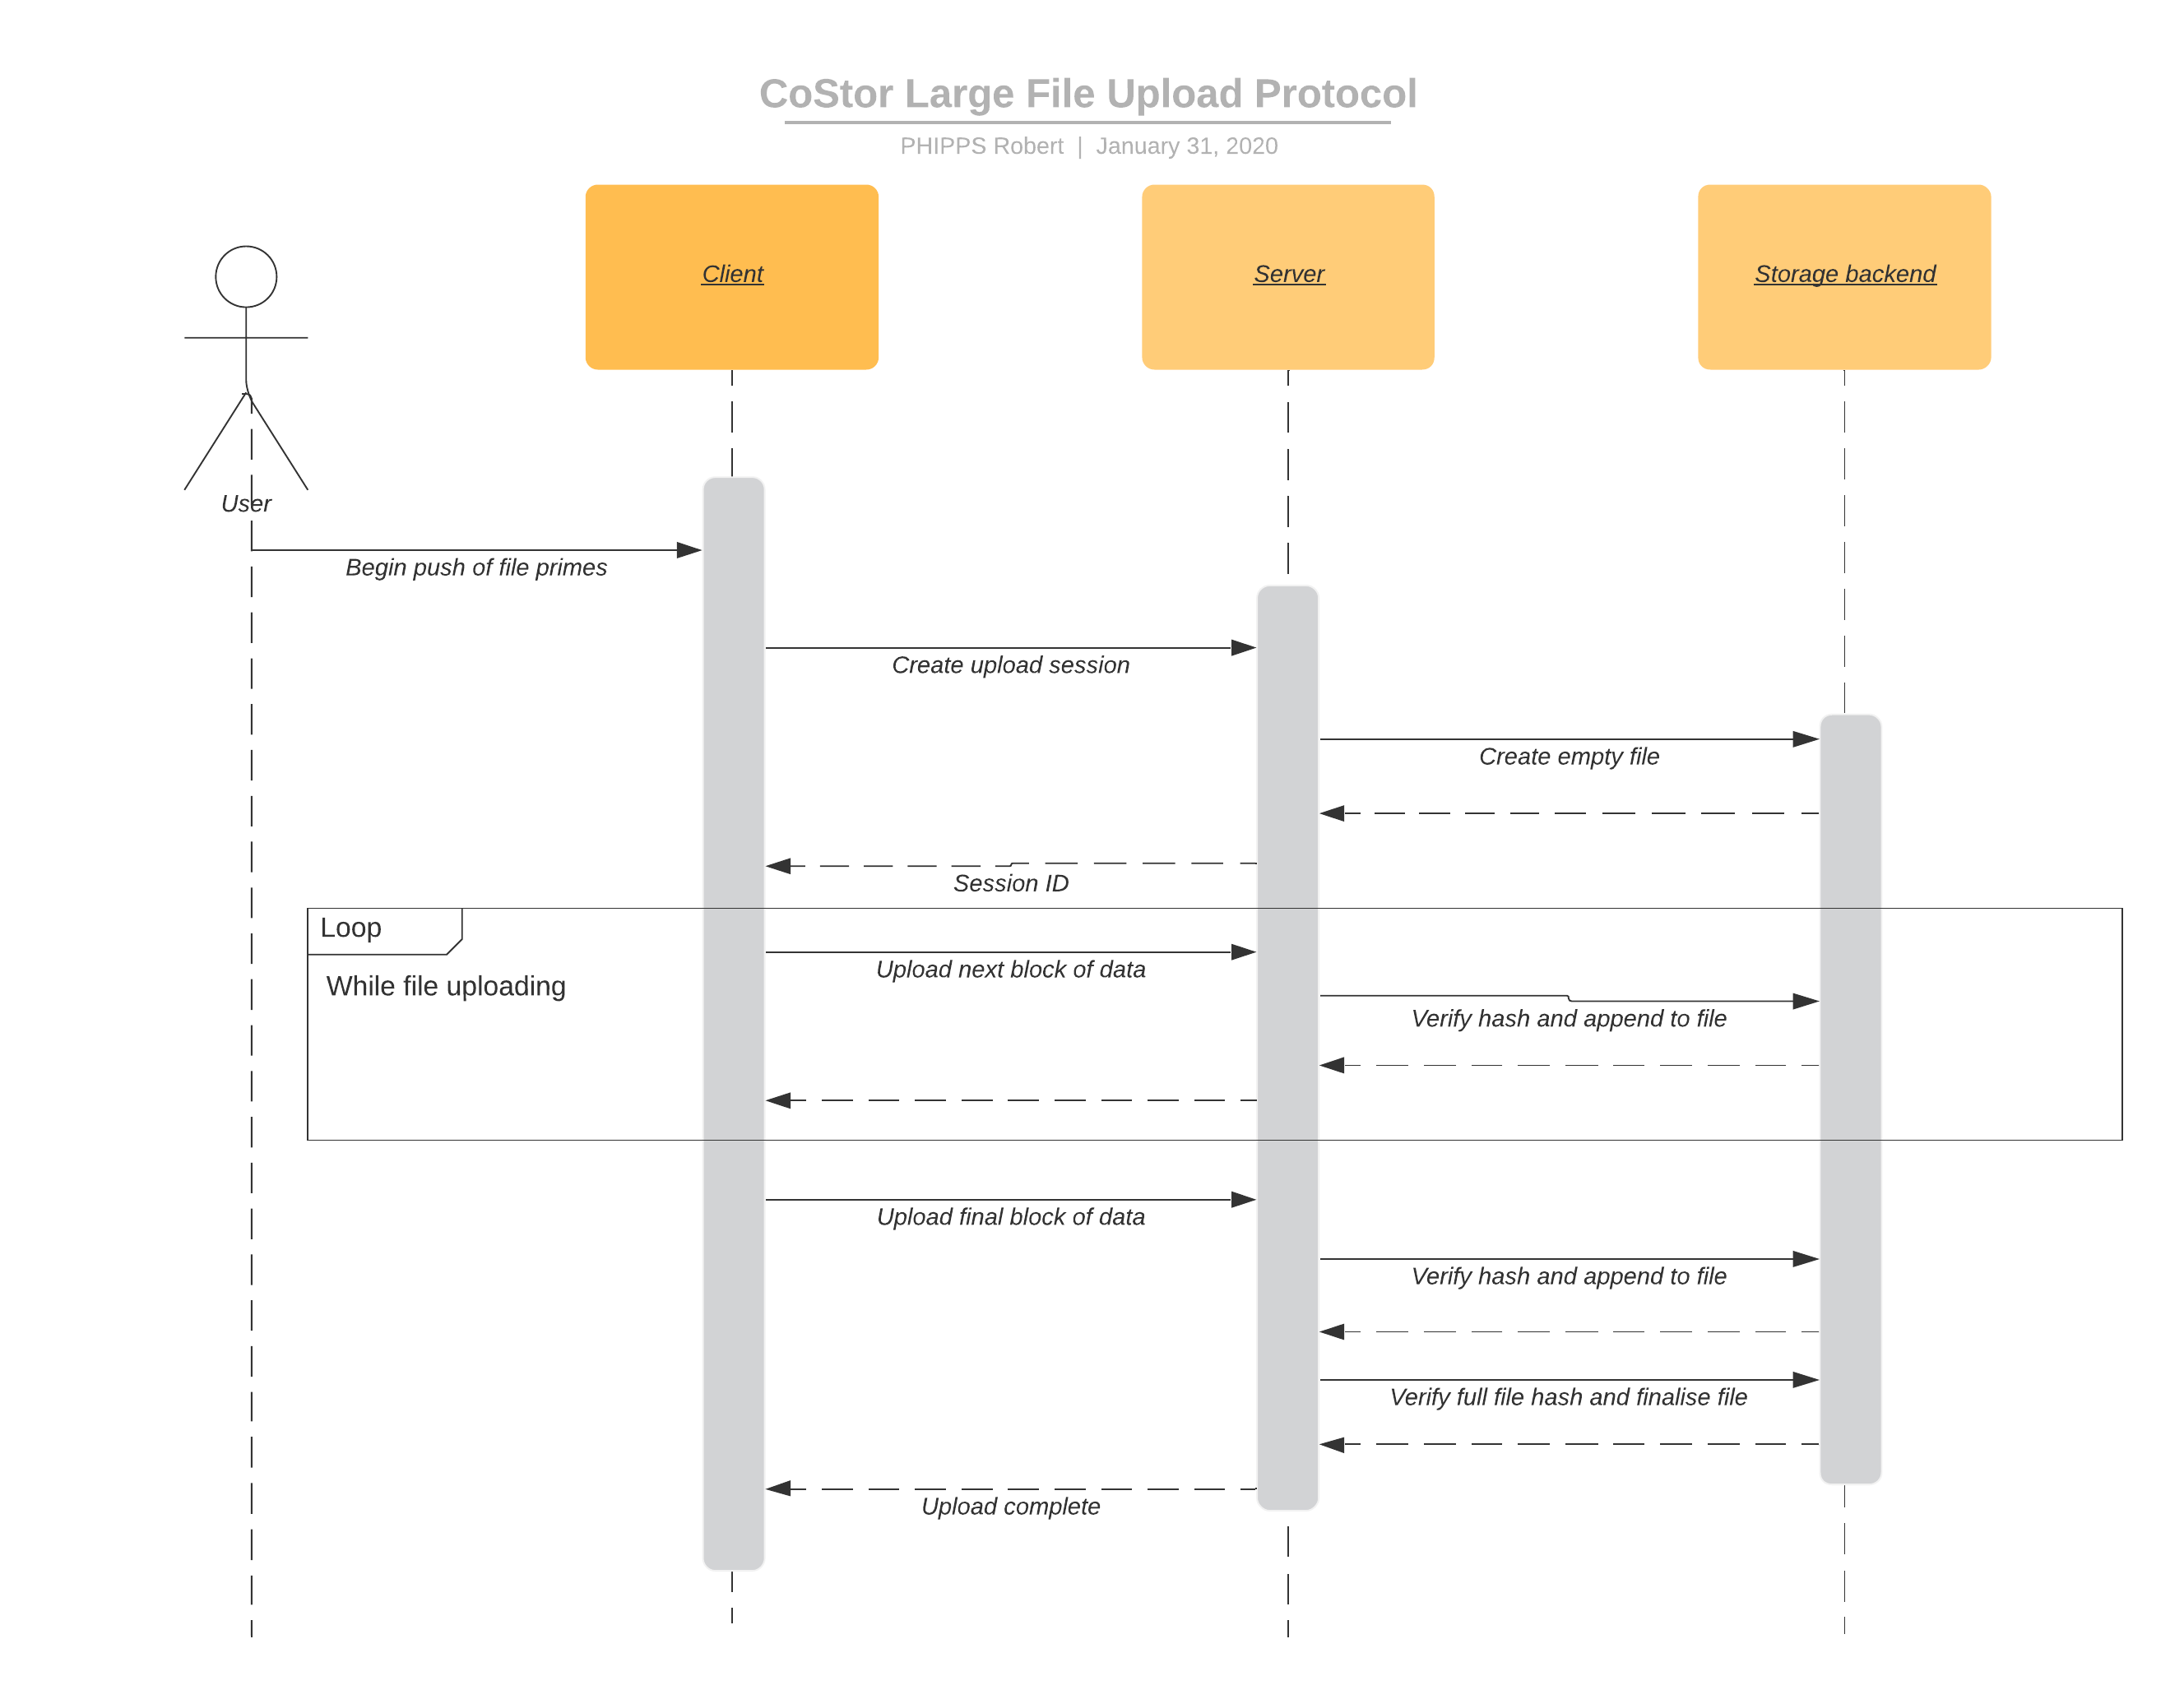
\includegraphics[width=1.1\linewidth]{img/lfileupload.png}
	\caption{UML sequence diagram for large file upload}
	\label{fig:lfileupload}
\end{figure}

Integrity is ensured by having the client create an "upload session" before pushing chunks of
files. This session includes the file hash and the number of expected parts. Each part is also 
uploaded along with its hash and sequence number, which is verified before the data is appended 
to the file in the server's filesystem. Once the final part has been received, the server 
checks the completed file against the hash given in the upload session before marking the file
as complete and closing the session.

Chunks can be uploaded over any period of time, and chunks for one file/session can be uploaded
interspersed with chunks from other files, the only constraint is that chunks for a session are
received in correct sequence order.

Should a chunk fail its upload, due to a verification error or network instability, the client
is able to retry this chunk once network has been restored, allowing uploads to be "resumed", at 
least to the resolution of the chunk size.

\section{SQL database and other backup plugins}

To facilitate safe and reliable backup of specialist server applications, it is necessary to perform
steps to either shut down or pause its processes before working with its underlying datastore. 
These would be implemented as plug-in modules to the client, which could be configured along
with other backup parameters.

Taking the example of Microsoft SQL Server, a database dump can be created with the following 
short SQL command that could be easily wrapped within in a PowerShell script:

\begin{figure}[h]
	\begin{minted}{sql}
	USE SQLTestDB;
	GO
	BACKUP DATABASE SQLTestDB
	TO DISK = 'c:\tmp\SQLTestDB.bak'
   		WITH FORMAT,
      		MEDIANAME = 'SQLServerBackups',
      		NAME = 'Full Backup of SQLTestDB';
	GO
	\end{minted}
	\caption{An example SQL script to create a backup from a running instance of the Microsoft SQL Server, source: Microsoft Docs\cite{mssql}}
\end{figure}

The below applications were investigated as candidates for backup plugin development:

\begin{itemize}
	\item Microsoft SQL Server
	\item MySQL server (Windows/Linux)
	\item Microsoft Active Directory Server\footnote{https://docs.microsoft.com/en-us/windows/win32/ad/backing-up-an-active-directory-server}
\end{itemize}

Unfortunately, the current implementation of CoStor client does not include support for such plugins, 
although integration should be trivial.

\section{Filesystem snapshots and integrity protection}

If the user intends to backup rapidly changing data which is always being accessed by another 
process (such as a operating system core files), it is necessary to ensure that files 
cannot change during the backup process. One way of achieving this is to create some form
of snapshot of the filesystem while the backup is running. This is currently being investigated
and will likely make use of LVM, Microsoft Shadow Copies and Time Machine on Linux, Windows and
MacOS respectively, however is non-trivial to implement given the differing systems available across
both the operating systems and filesystem types.

The current implementation assumes the subtree being backed up is not going to change during the
backup process.

\clearpage

\section{The HashTreeMaker}

This class is the engine behind the creation of the filesystem metadata snapshot, and builds
simple objects that can be stored in the relational databases used by CoStor. As part of the 
object creation, metadata is pulled from the \texttt{os.stat} command, and unique ids are generated
based off SHA-1 hashes of both the metadata, and, in the case of files, binary data.

An early standalone implementation of the HashTreeMaker used during development to dump directory
structure to JSON for debugging is located in the \texttt{costor\_hasher} directory, however the
version used within \texttt{costor\_client} has been through many more iterations as it was integrated
with the rest of this application.

\begin{figure}[b]
	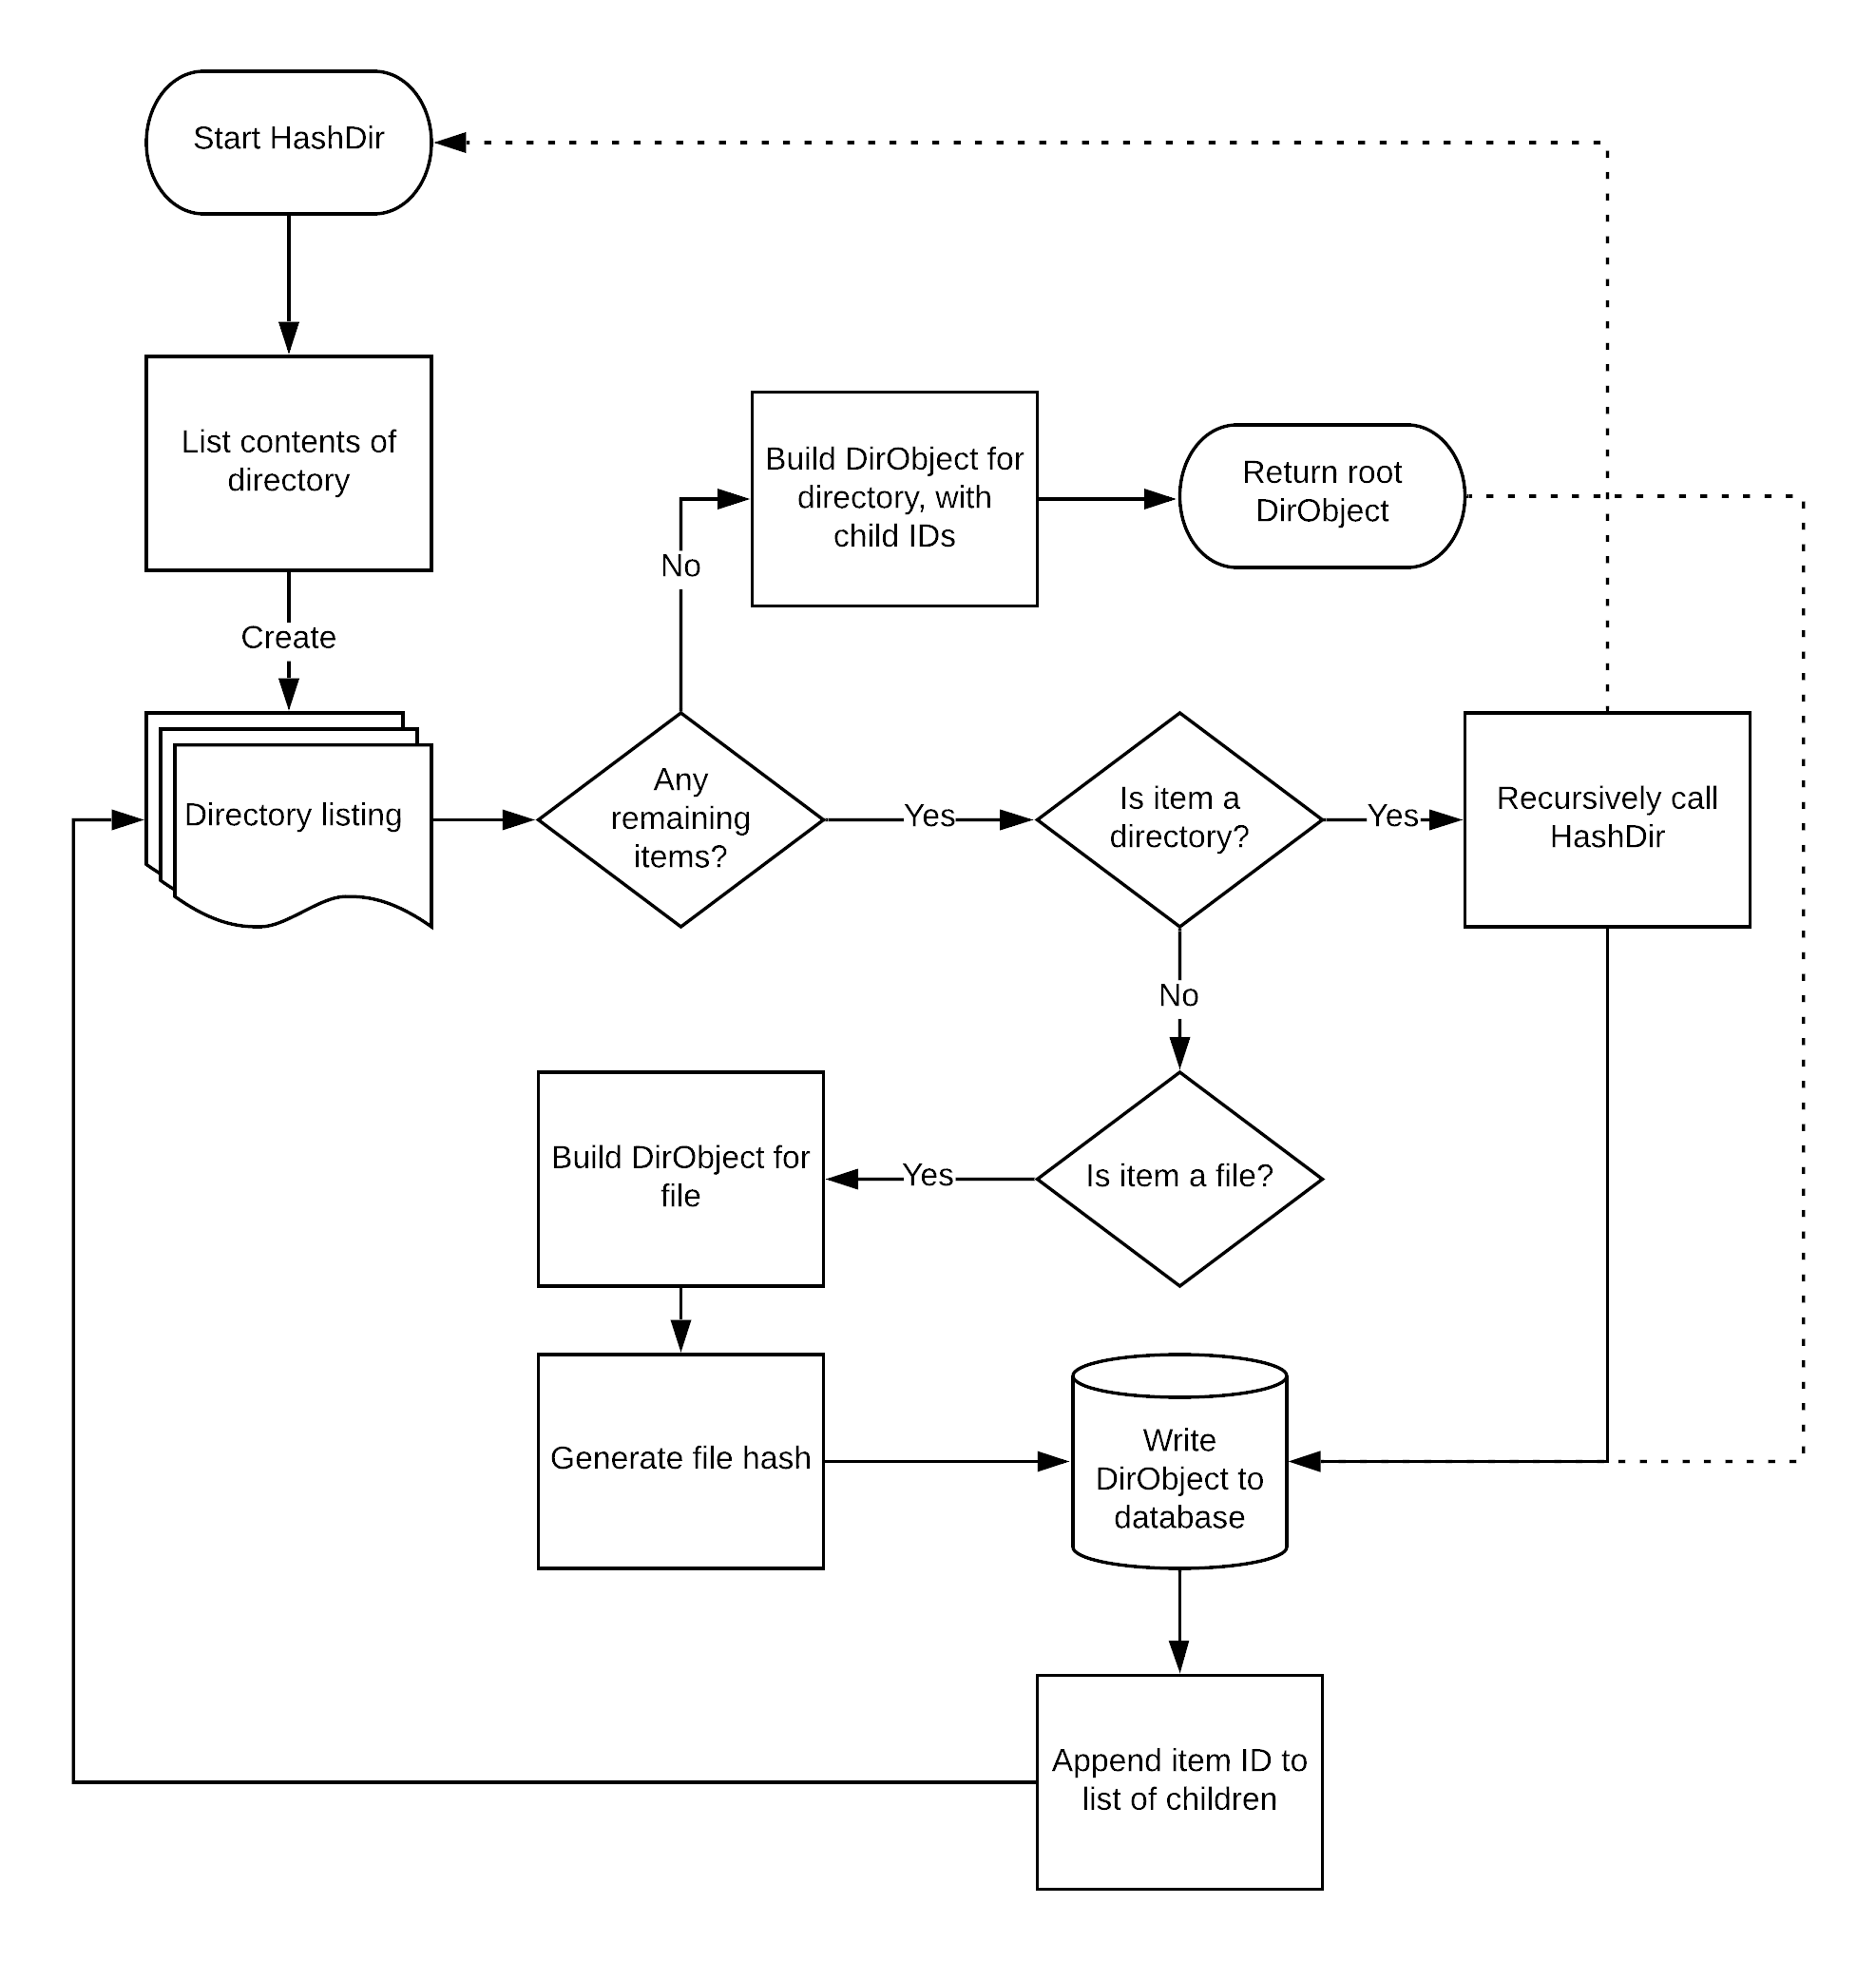
\includegraphics[width=\linewidth]{img/hasherflow.png}
	\caption{Flowchart of process for creating DB representation of directory tree}
	\label{fig:hasherflow}
\end{figure}

All database objects are managed by PonyORM\footnote{PonyORM: an advanced object-relational mapper \url{https://ponyorm.readthedocs.io}}
- the most important entity definitions (database models) are shown in Figure \ref{fig:clientmodels}.
These definitions make heavy use of foreign key relations to simplify movement around the data.

The \texttt{Object} class represents the metadata for a single filesystem object, and if there is 
binary data associated with the object (in the case of regular files), the path of the canonical
version (which can be shared between multiple objects) is stored with its SHA-1 hash as a \texttt{Prime}.
These objects are created from the \texttt{DirObject}s built by the \texttt{HashTreeMaker}. CoStor
generates a unique identifier for each \texttt{Object} from the SHA-1 digest of the object path concatenated 
with the object hash.

The hashes for \texttt{DirObject}s are generated by the \texttt{gethash} function within the \texttt{DirObject} 
class. This allows the hash to be returned without modifying the object instance, and inadvertently changing its 
hash. Object hashes are calculated from the SHA-1 digest of the binary data in the case of files, and from the 
digest of the concatenation of the name, path, stat metadata and the sorted string representation of its 
children's hashes in the case of a directory. The function is shown in Figure \ref{fig:dirobjgethash}.

\begin{figure}
	\begin{minted}{python}
	def gethash(self: DirObject):
        if self.type is "file":
            return self.hash
        elif self.type is "dir":
            shastring = self.name + self.path + str(self.stat)
            childhashes = str(sorted(self.children))
            return sha1str(shastring + childhashes)
	\end{minted}
	\caption{Method to generate file hash from \texttt{DirObject} (costor\_client/hasher.py)}
	\label{fig:dirobjgethash}
\end{figure}

\begin{figure}
	\begin{minted}{python}
    # a specific run of this application
    class Snapshot(db.Entity):
        id = PrimaryKey(int, auto=True)
        timestamp = Required(datetime)
        complete = Required(bool)
        synced = Required(bool)
        objects = Set('Object', reverse='snapshots')
        root = Required('BackupRoot', reverse='snapshots')
        topobject = Optional('Object', reverse='topobjectfor')
        parent = Optional('Snapshot', reverse='child')
        child = Optional('Snapshot', reverse='parent')
        primes = Set('Prime', reverse='snapshots')
    
    # anything included in the backup tree
    # type can be "file" or "dir" (or "sym")
    class Object(db.Entity):
        id = PrimaryKey(str)  # sha(path+hash)
        hash = Required(str)
        name = Required(str)
        prime = Optional('Prime', reverse='objects')
        path = Required(str)
        type = Required(str)
        stat = Required(str)
        children = Set('Object', reverse='parent')
        parent = Optional('Object', reverse='children')
        snapshots = Set('Snapshot', reverse='objects')
        topobjectfor = Optional('Snapshot')
        depth = Required(int)

    # file path to object hash mappings
    class Prime(db.Entity):
        filehash = PrimaryKey(str)
        paths = Set('Path', reverse='target')
        firstseen = Required(datetime, sql_default='CURRENT_TIMESTAMP')
        lastseen = Required(datetime, sql_default='CURRENT_TIMESTAMP')
        objects = Set('Object', reverse='prime')
        snapshots = Set('Snapshot', reverse=None)
	\end{minted}
	\caption{PonyORM database entity definitions for client (costor\_client/db.py)}
	\label{fig:clientmodels}
\end{figure}

\chapter{Server and datastore implementation}

\section{Overview}

CoStor server is a Django based web application, that can be deployed within Docker for easy
installation and upgrades. It not only provides the backup API endpoints used by the Client
software to actually push snapshot data to the server's storage, but also a web UI for 
management and monitoring, as well as frameworks to allow replication of backup data between
instances of the server over a standard HTTPS connection.

To allow larger tasks (such as backup archive generation) to run asynchronously of the HTTP
requests to the web server, it was planned to make use of a task broker such as Celery\footnote{\url{http://www.celeryproject.org}} 
, however this is not implemented within this version of CoStor.

\section{High-level data architecture}

To allow all machinery to be as generalised as possible, all possible file system objects are stored
as generic \texttt{Object} objects. These can represent files, directories or symlinks. Each object
holds a globally unique ID, path information, the hash of the object's contents, child and parent 
relations, the path and link to a \texttt{DbFile} object or "prime" in the case that the object is
a file, with the prime representing the binary data of that file on the CoStor server's filesystem.

These objects are then related to their associated "snapshot" or backup session, backup root directory
and the agent (or CoStor client identity) that the backup originated from.

\section{Server metadata database and filestore}

All data on the CoStor server is stored within the context of the Django ORM, to allow easy access
to all objects using the powerful Object APIs provided by the ORM. The backup data is stored in the
following database models:

\begin{figure}[h]
	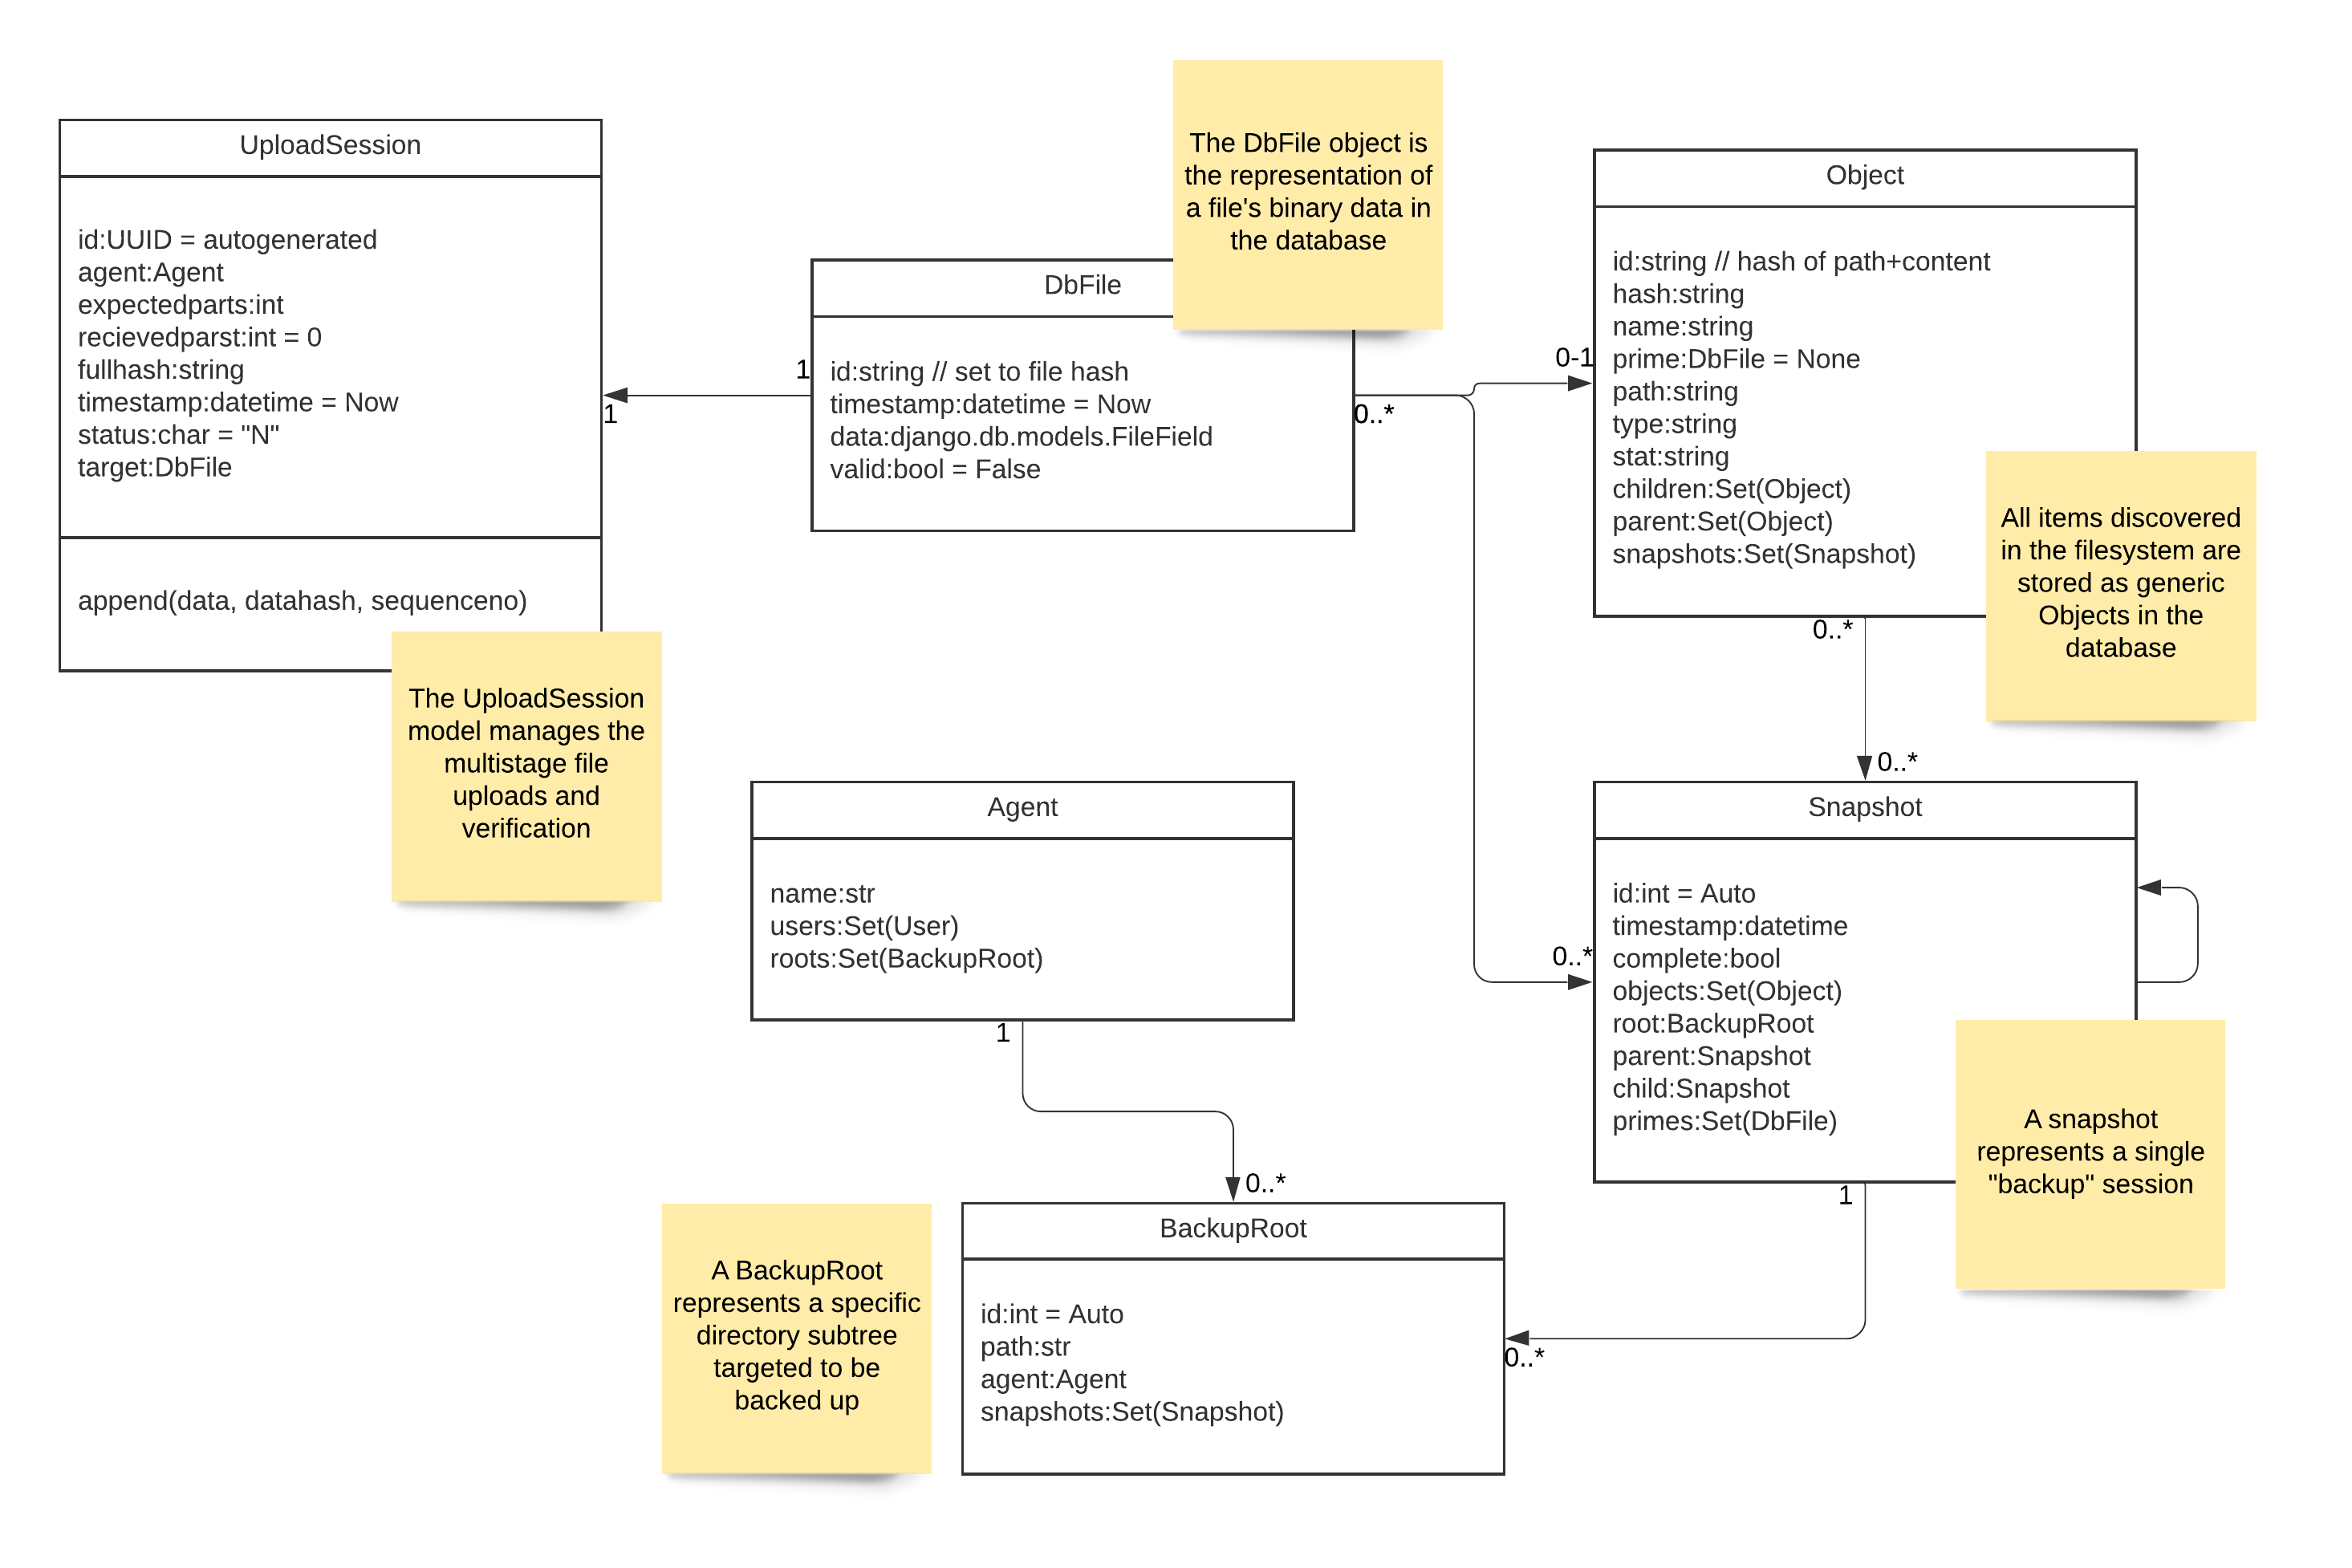
\includegraphics[width=0.82\paperwidth]{img/serverfileuml}
	\caption{UML of Django ORM models used to manage backup data}
	\label{serverdjangofileuml}
\end{figure}

File data is stored wrapped within a \texttt{django.orm.models.FileField} attached to the DbFile 
object and stored on the filesystem of the CoStor server at a location defined by the config file,
with the filename being the object's ID.

\section{Management UI}

CoStor server makes use of the built in Django Admin package for management of database objects 
and user permissions. There is additionally a custom frontend used to browsing registered agents,
their backup tasks (backup roots), snapshots and the file trees of each snapshot.

Once a snapshot has been located by the user, there is the option to download a copy of that
snapshot's contents as a \texttt{tar.bz2} archive.

\begin{figure}
	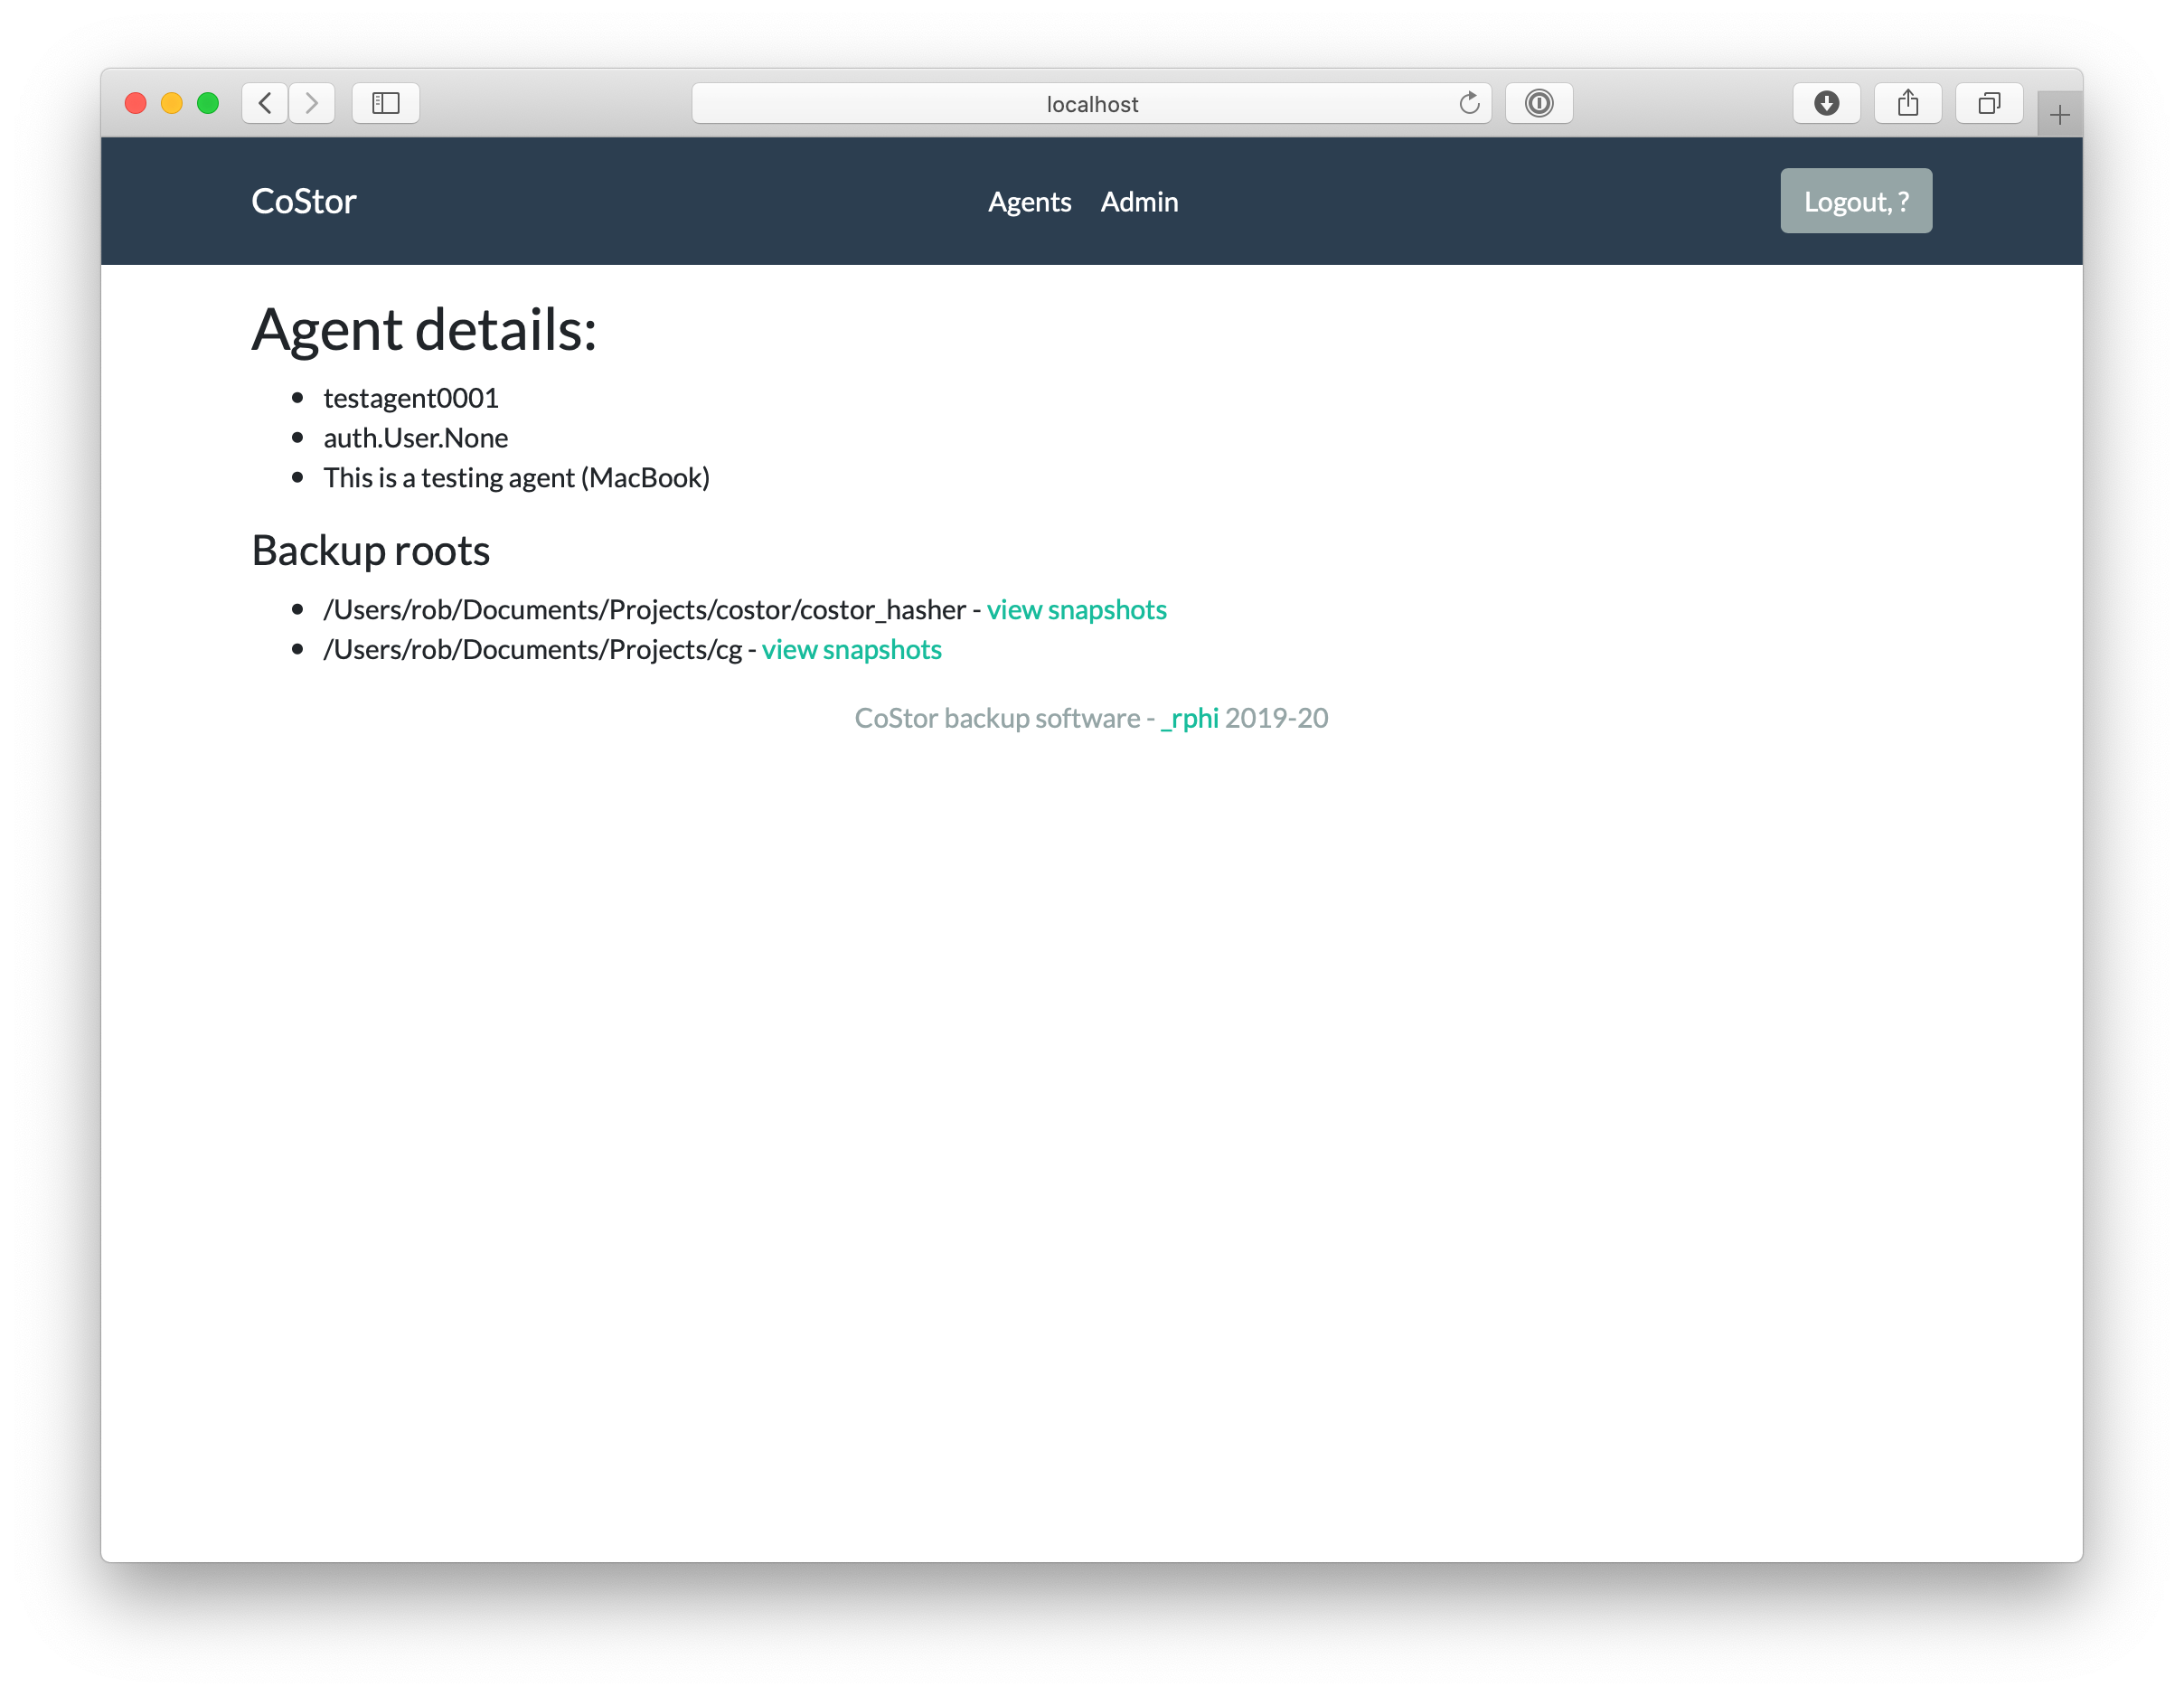
\includegraphics[width=0.75\linewidth]{img/screenshots/agent}
	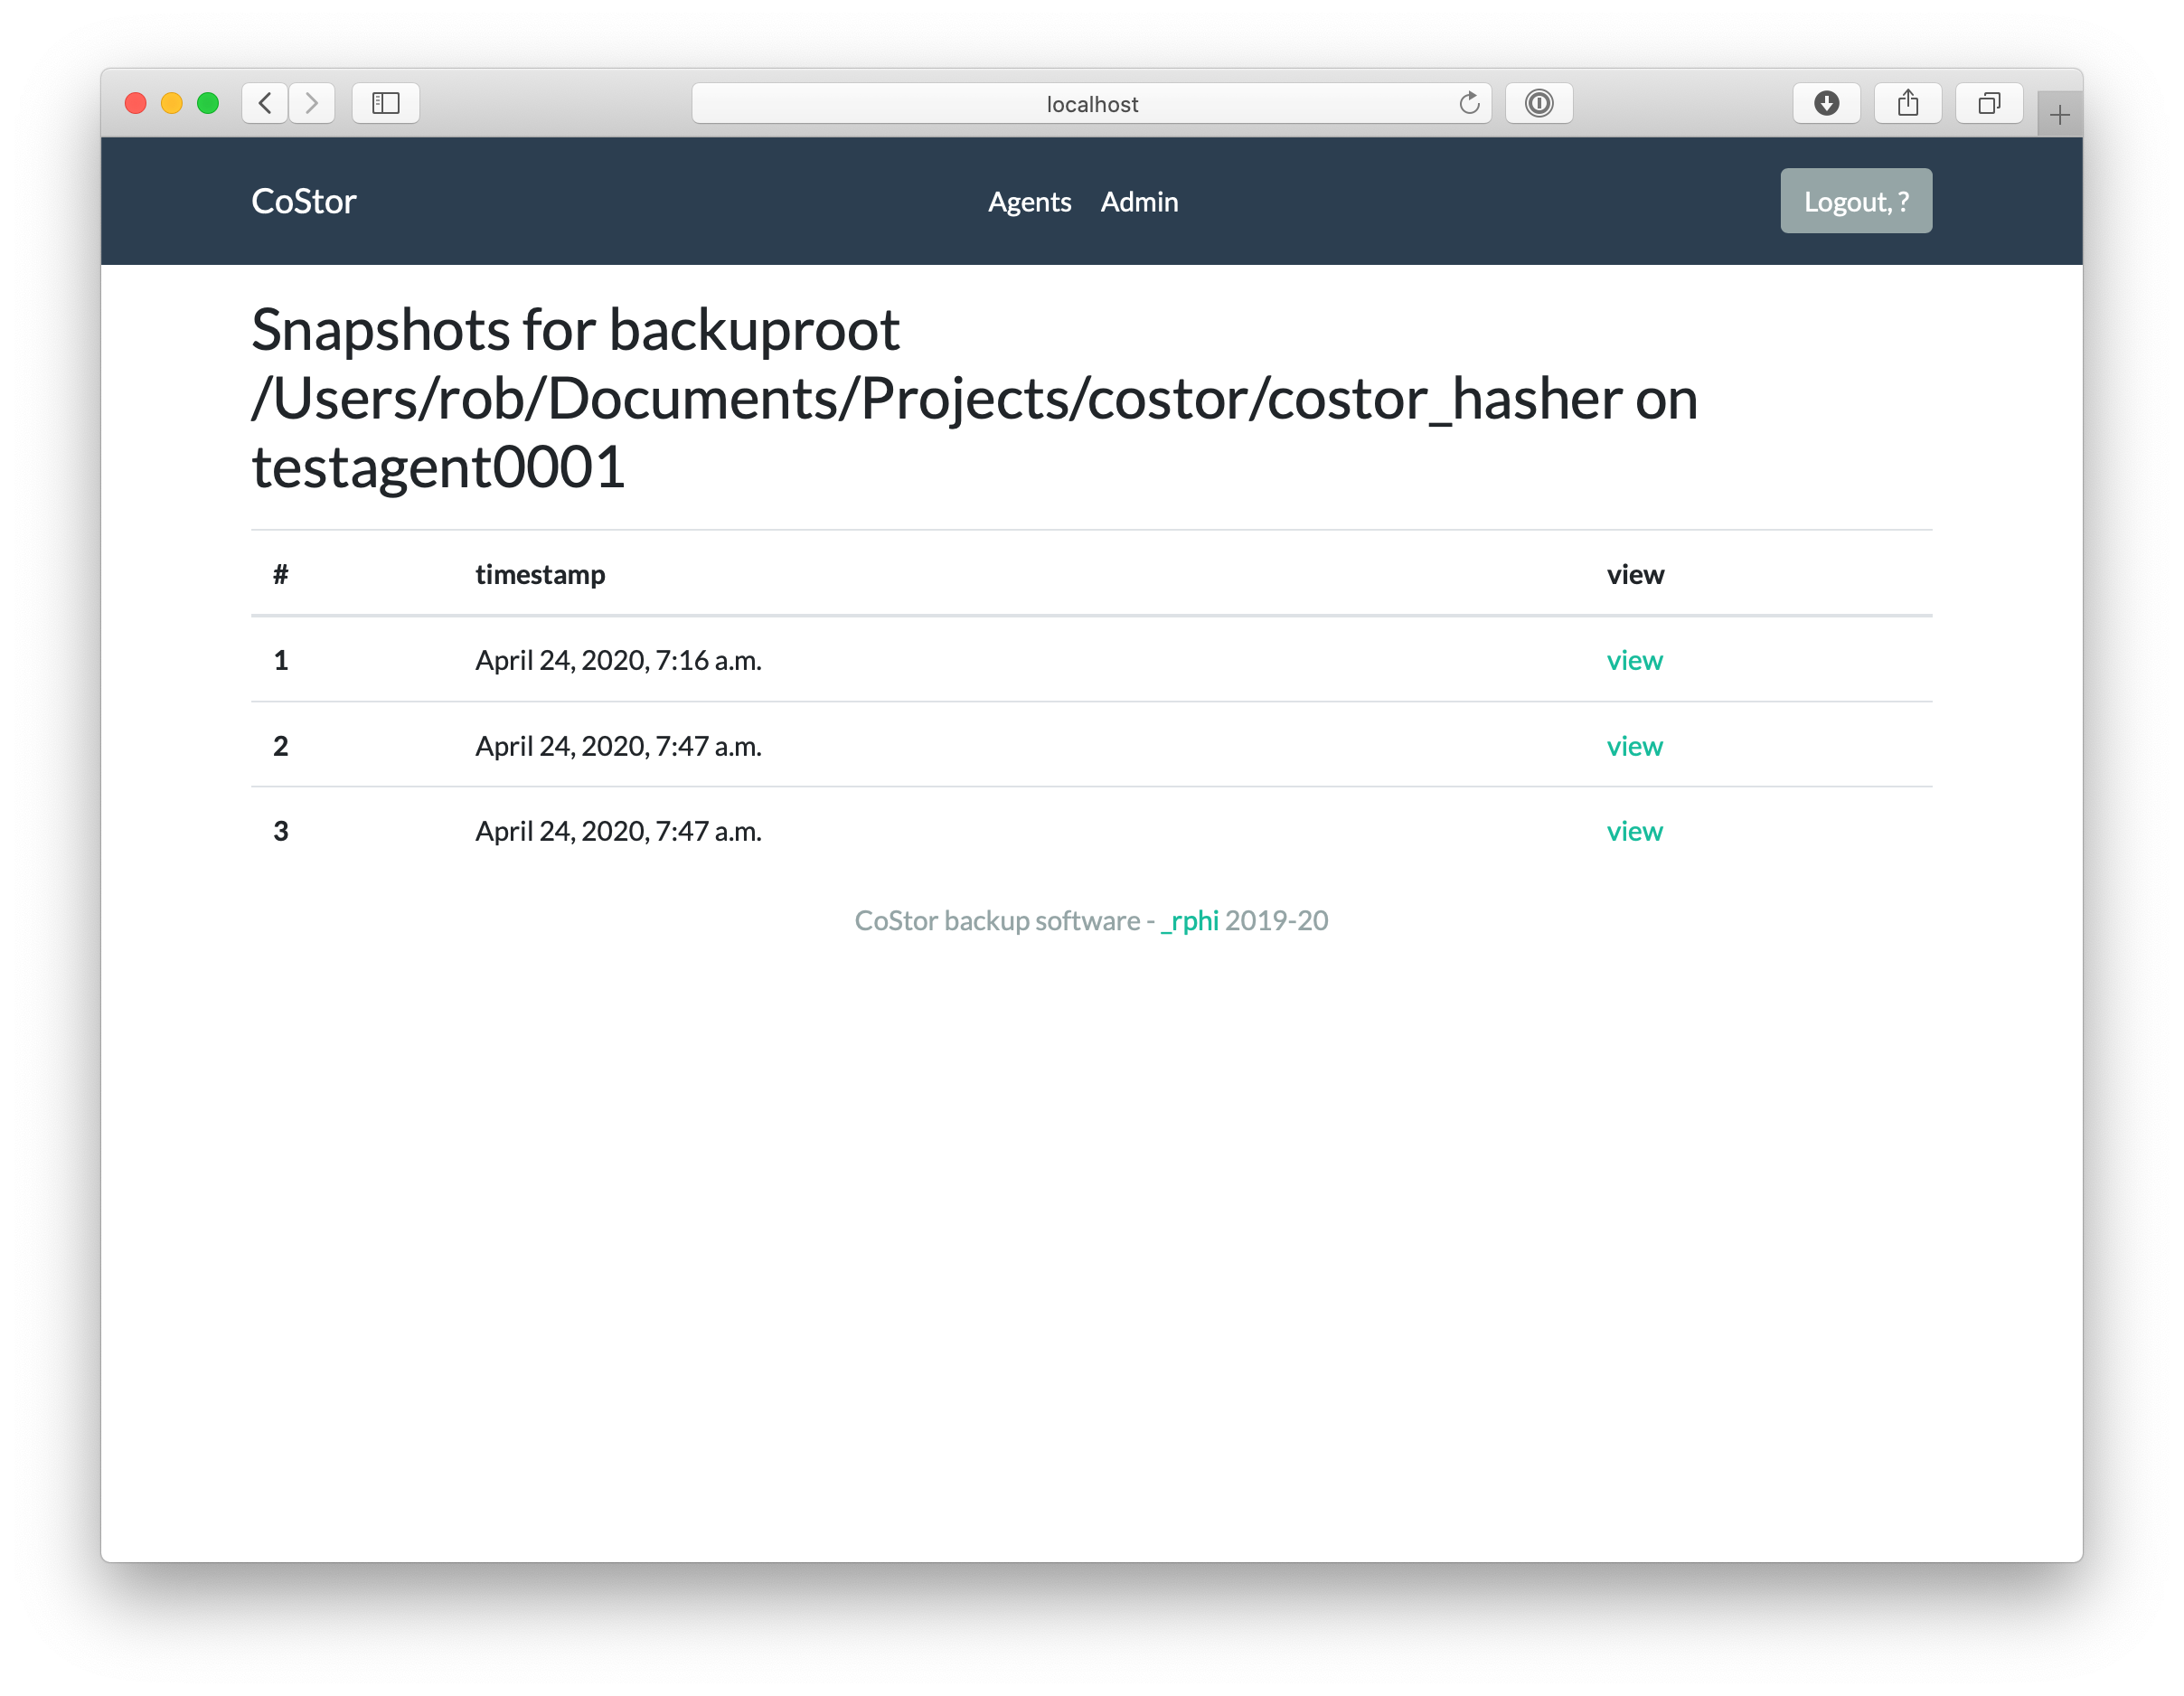
\includegraphics[width=0.75\linewidth]{img/screenshots/snapshots}
	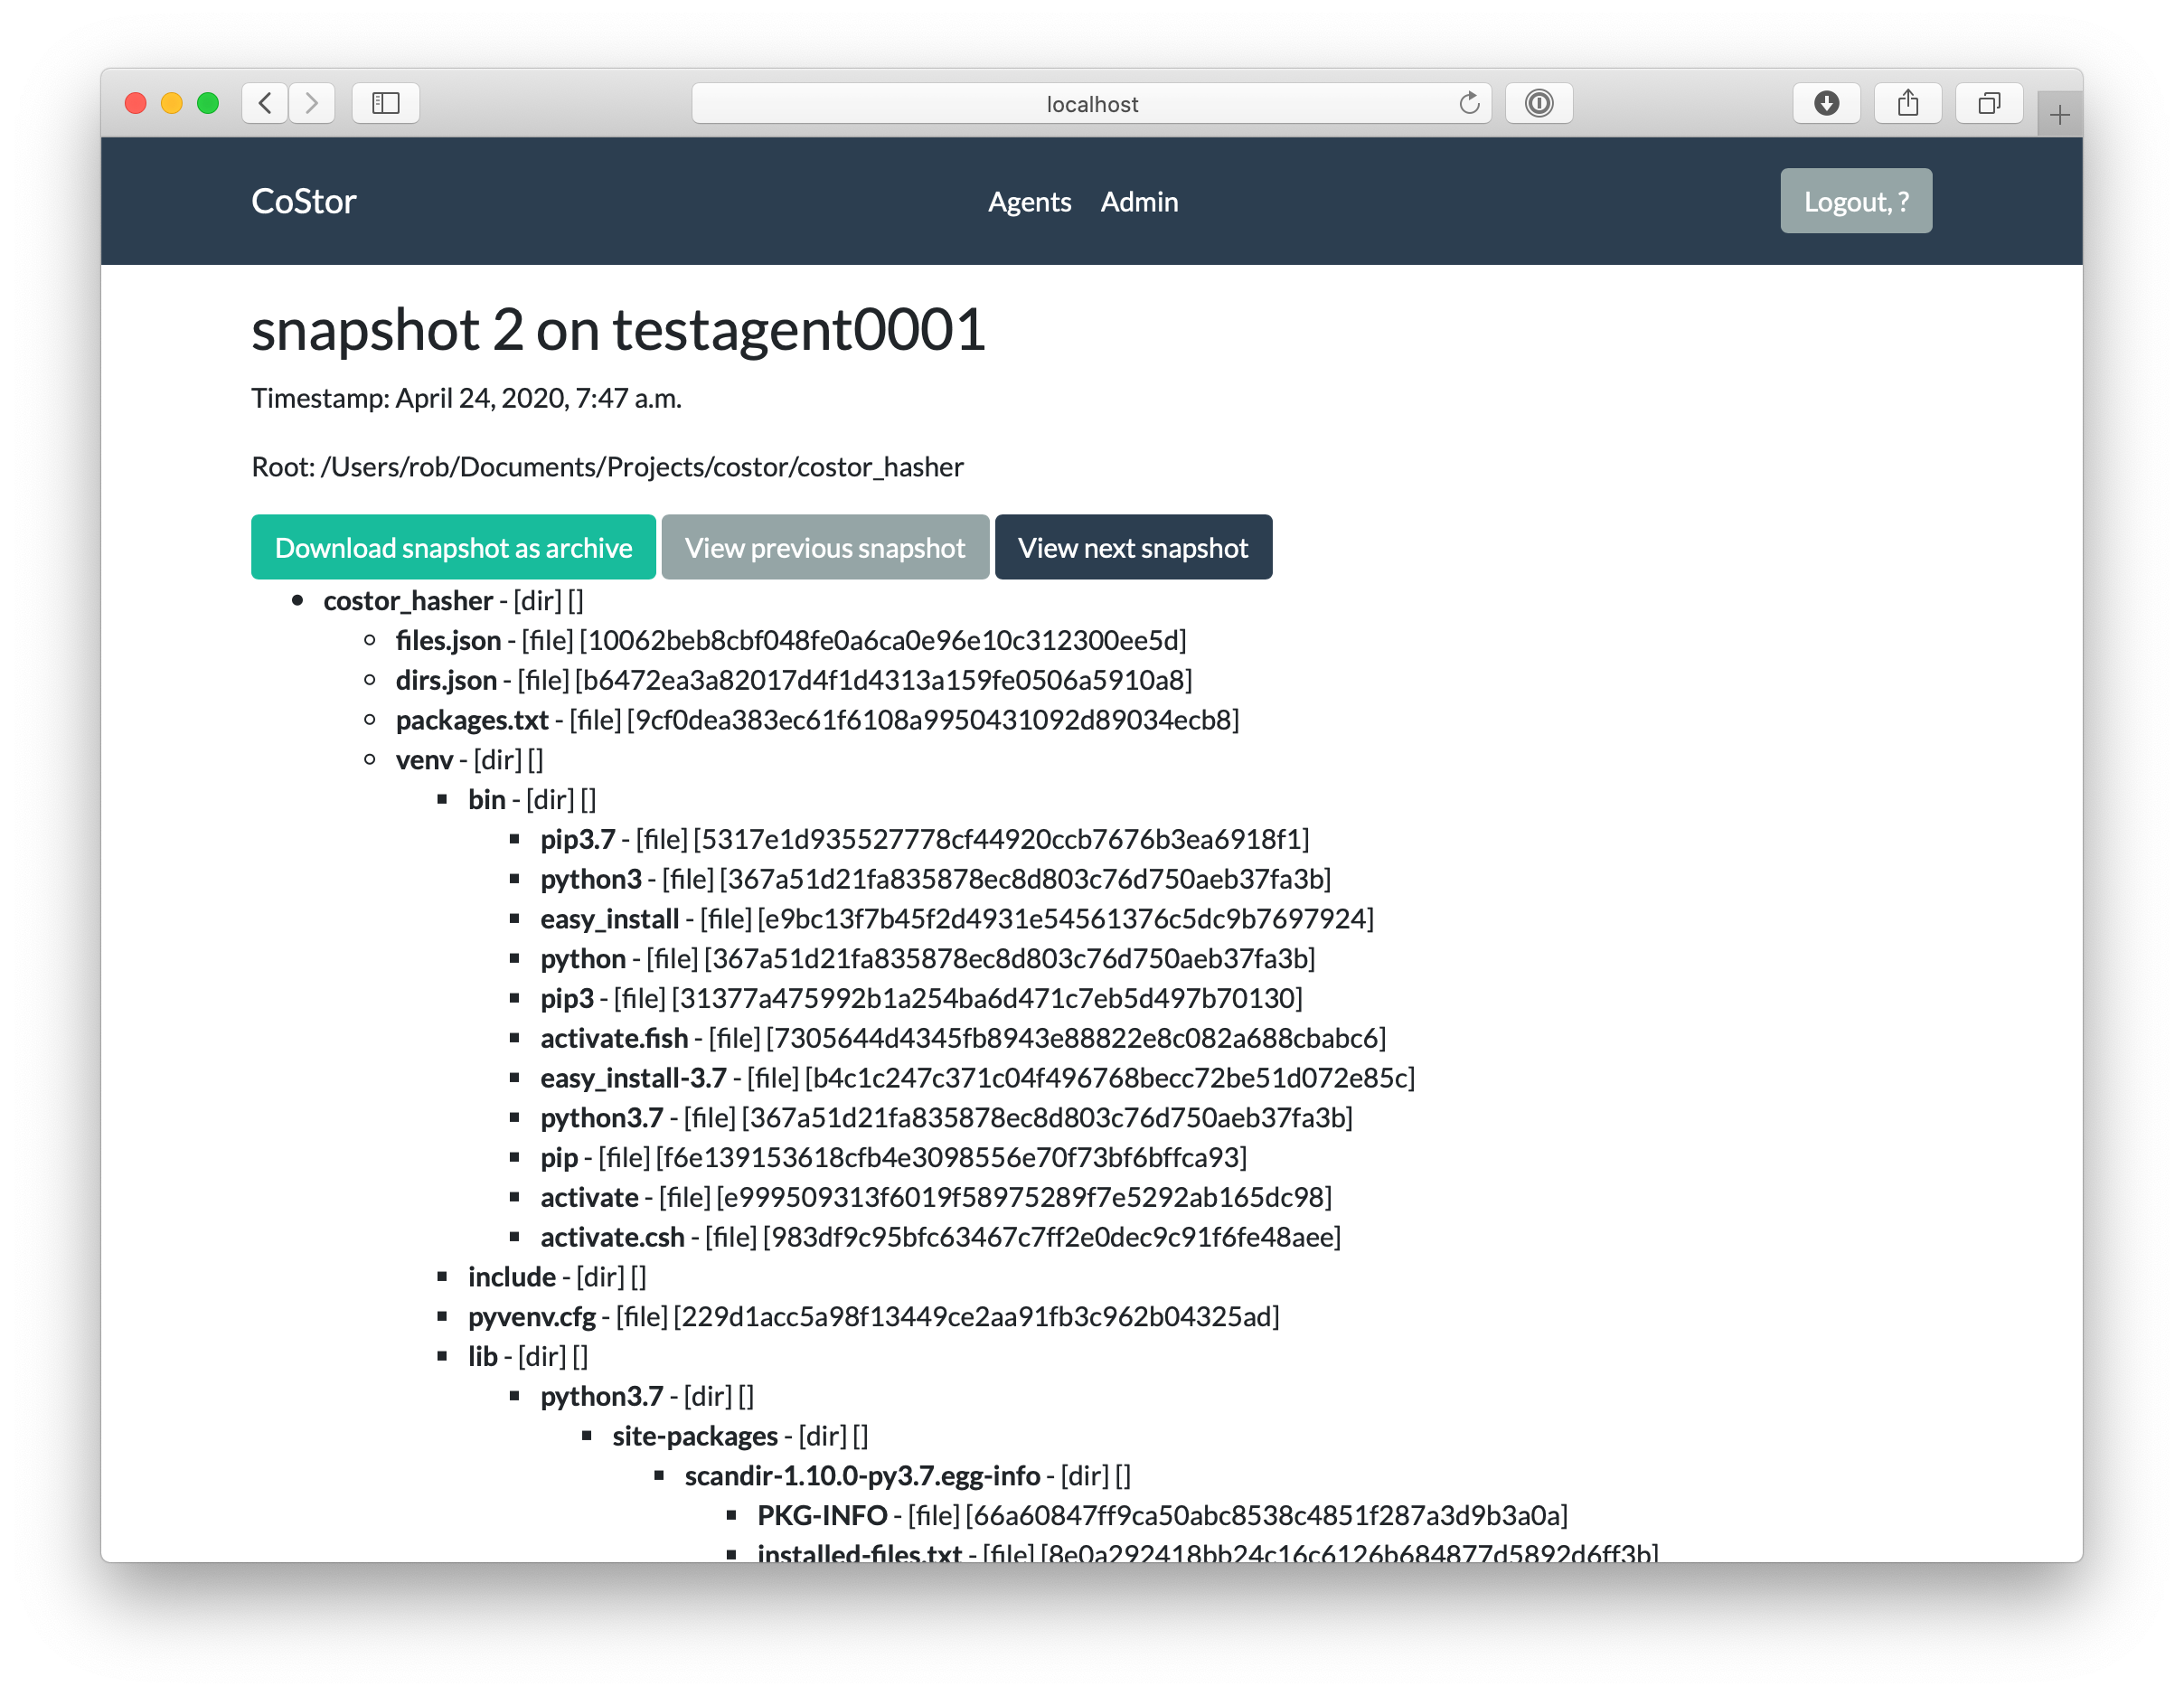
\includegraphics[width=0.75\linewidth]{img/screenshots/snapshot}
	\caption{Screenshots of the CoStor browser}
	\label{fig:browser}
\end{figure}

\section{Restoring backups}
\label{sec:restoringbackups}

\subsection{Direct (local) restore}

These are the most straightforward of restores, the administrator simply has to find a directory
or object within the data browser interface  for an agent and snapshot within the web UI (Figure \ref{fig:browser}) for their 
site's local instance of CoStor server, before requesting a restore package be generated. CoStor 
then re-builds the original directory tree selected from database objects and creates an archive
of the backup which can be downloaded and restored manually.

This is built by recursively traversing through the directory tree, starting from the object defined in the 
snapshot as the \texttt{topobject}. First the directory structure is rebuilt in a temporary 
directory (\texttt{/tmp/costordownload/<snapshotid>}), with file permissions, UIDs and GIDs 
restored from the object's \texttt{stat} attribute which was generated from the \texttt{os.stat}
package when the client initially catalogued the file.

Once the tree is complete, this is archived into a \texttt{tar.bz2} package, the temporary 
uncompressed structure is removed and the archive is delivered to the user's browser.

This method does have some downsides:

\begin{itemize}
	\item An in place restore (eg from a context menu) is 
		obviously impossible, although it would require considerable research to be able to reliably
		hook into the supported OS' file explorer context menu APIs.
	\item The user cannot currently
		restore their own data, the archive would need to be created by the administrator.
	\item This archive is generated synchronously on the web server thread. Obviously with very
		very large backups, it would be far more sensible to move this logic into an asynchronous
		task runner.
	\item It is not possible to request a single file from a snapshot, nor can you view version
		history for a single file
\end{itemize}

Ultimately, it would make sense to implement a self-service restoration interface within the CoStor
client, which could vastly improve the end-user experience.

\subsection{Remote (disaster recovery) restore}

\textit{\textbf{NOTE:} the functionality detailed below has not been implemented in this version of CoStor, as there is no completed support for multiple-instance replication. It is however left as context to other architectural decisions made throughout CoStor}

\subsubsection{Using offsite instance to restore individual snapshots}

In the event that the instance of CoStor has failed for the site that is being backed up, it should
be possible to restore a backup from another site's instance of CoStor.

\begin{enumerate}
	\item As all metadata for replicated sites is encrypted, a valid master decryption key must
	be provided to the server being used to restore a backup. This is checked against the master
	federation database, which is replicated to all servers within the group.
	\item The server then identifies which CoStor servers contain copies of the metadata 
	databases for the requested site (using the global master federation database), and requests
	that metadata be replicated to itself if the data is not already available locally.
	\item Finally, the server decrypts the replicated metadata for the requested agent and 
	snapshot, allowing the administrator to generate a restoration archive using the same
	method for a local restore: browsing the directory tree and selecting required sub-trees
	to be restored. File "primes" or binary data blocks are decrypted on the fly before being 
	written to the restoration archive.
\end{enumerate}

\subsubsection{Restoring entire datastore from offsite to replacement CoStor server}

In the event that the hardware running CoStor has to be replaced, it should be possible to replicate
all data for that site back to the new server from the replicated copies across other sites.

\begin{enumerate}
	\item The new instance should be configured with the same ID, encryption key and access 
	token as the original server, to re-enroll it into the network. The master federation 
	database will then be replicated to this new server.
	\item The new (replacement) server can then request that all replicated data from its site
	is returned to its local storage, and will decrypt each package as it arrives to rebuild
	the server's original state.
	\item Once all data has been restored to the server, the restoration continue as outlined
	in the direct (local) restore procedure.
\end{enumerate}

\section{Automated maintenance}

Due to the use of the Django ORM for management of all data storage, including file storage
of object primes, CoStor is very resilient to datastore inconsistencies. All database models
are defined with \texttt{on\_delete} actions to allow the database to automatically prune
itself once a snapshot, backup root or agent is removed.

All data entry is additionally validated before being written, to ensure the database cannot
contain invalid data.

\chapter{Multi-site replication}

\textit{\textbf{NOTE:} the functionality detailed below has not been implemented in this version of CoStor. It is however left as context to other architectural decisions made throughout CoStor}

The data to manage multi-site restores should be stored in a globally replicated database, which 
contains information such as the replication status of all snapshot directory trees and file 
"prime" objects, anonymised agent ID to site mappings, and synchronisation job objects to track
when and to where objects are replicated.

Each site would manage its own replications, and respond to replication requests from other servers
within the network. All objects are identified globally by the hash of their contents, and 
database objects would be replicated as encrypted JSON documents. File "primes" would transferred
between sites using the large file upload protocol used by the clients (outlined in Figure \ref{fig:lfileupload})

The overall goal of the replication system would be to ensure there are at least two redundant, offsite
copies of all data. This would be performed by selecting replication targets randomly, weighted by 
free disk space, and by incrementally scheduling the replication tasks during a configured
maintenance window (normally overnight when the network is quiet).

\section{Data distribution and sharding}

Each server would choose two sites to distribute its data across to. This means that each instance
of CoStor would be holding the backup data of its own site, plus compressed copies of two other
sites' backups.

\section{Replication management database}

To allow all federated instances of CoStor to collaborate on managing replication tasks, and to
enable restoration from federated data even if the master database for that site is unavailable 
(in the event of a server failure), the replication data would be synchronised across all servers.

All operations on these database tables are wrapped such that an API request is made to all other
servers to update them immediately. Additionally, before a replication task commences, a full
sync is requested to ensure that all servers contain all objects. To allow the servers to easily
verify data integrity across nodes, all entries in this database have a UUID and are write only. 
When a sync is triggered, the server sends a request to all other CoStor servers with the full 
list of object IDs. If any IDs are missing, each server requests copies of these. If any server
finds that it has an object with an ID that isn't in the list, it can assume that object has been 
deleted and will purge it from its own copy of the database.

This database contains information such as which backup Objects and file "primes" 
(Figure \ref{serverdjangofileuml}) have been replicated to which locations, current status of all
nodes, and basic information on which sites own which agents and snapshots. This database 
\textbf{must} contain all the information needed to initiate a restore in the event of a remote 
disaster recovery restoration (Section \ref{sec:restoringbackups}). As only the server to
be modifying data relating to a site is the server located in that site, there is no risk of 
requests interfering with each other.

As almost every object in CoStor is referenced by a unique and anonymous ID, there is minimal 
risk in sharing this data with other servers.

\section{Securely synchronising data}

\large \textit{"How do we share data across sites without risking breach of confidentiality?"}
\normalsize

To enable the backup databases to be replicated securely, replicated data is stored using a modified
subset of the standard database objects used by the local backups (Figure~\ref{serverdjangofileuml}).

The actual DbFile objects do not require changing, as the data is already stored encrypted, and thanks
to the use of convergent encryption, the ID (or hash) of all of these objects is already the same as
those stored from the target server's local backups. The Object class is modified such that the name,
path and stat fields are stored as encrypted strings, but as the IDs, agent and snapshot IDs are unique
across sites, as well as being anonymous, these foreign keys can continue to be used.

\section{Efficiently transferring data}

We also need a way to transfer that data between hosts. As we already have serialisers for the 
database models thanks to the Django Rest Framework, it makes sense to re-use these to transfer 
database objects as JSON data. This also allows us to combine multiple entries into one large
request, as an entire snapshot's worth of data is still fairly small.

For file primes, if they are not already present on the target server, we can give these a quick bit
of compression using something fast like LZ4\footnote{\url{https://github.com/lz4/lz4}} to compress
each object before transmitting it using a modified version of the large file protocol utilised by
the client, described in Figure~\ref{fig:lfileupload}. These can then be decompressed and added to that
site's local DbFile store, where they may come in useful for local backups as well.

\chapter{Testing and evaluation}

The most important goal of a backup system is the ability to accurately first store, and then reproduce
a copy of the backup target from its datastore.

For the purpose of testing, the \texttt{cores\_hasher} directory within the project repository was set
as the backup root, and CoStor client was run to generate a backup to the server. This backup was 
downloaded as a \texttt{tar.bz2} from the CoStor management UI, and extracted alongside a copy of
the \texttt{cores\_hasher} test directory.

At first glance, it would be sensible to create a matching \texttt{tar.bz2} archive of the test files
locally, and binary diff that against the archive given to us by CoStor. Unfortunately, this is not
likely to be successful, as modification and creation timestamps are not preserved by the backup 
process.

The two copies of the test directory were compared using the GNU diff tool, using the \texttt{--recursive}
flag to allow it to traverse all the way through the tree. Running this tool confirmed both
directories were identical, which concludes that the data must be the same.

As this is a fairly small dataset, file permissions and groups were also checked by hand, and
the restored copy of the directory contained all of the correct metadata.

Although it would be worthwhile to perform more comprehensive testing on a larger directory tree,
performing all testing had to be completed locally on the development MacBook, as any work on
remote servers would be rendered fairly difficult thanks to my uplink being provided by a fairly flaky
cellular data dongle. Additionally, the current synchronous archive generation method used by the web
UI would unlikely be very performant with larger backups.

\begin{figure}
	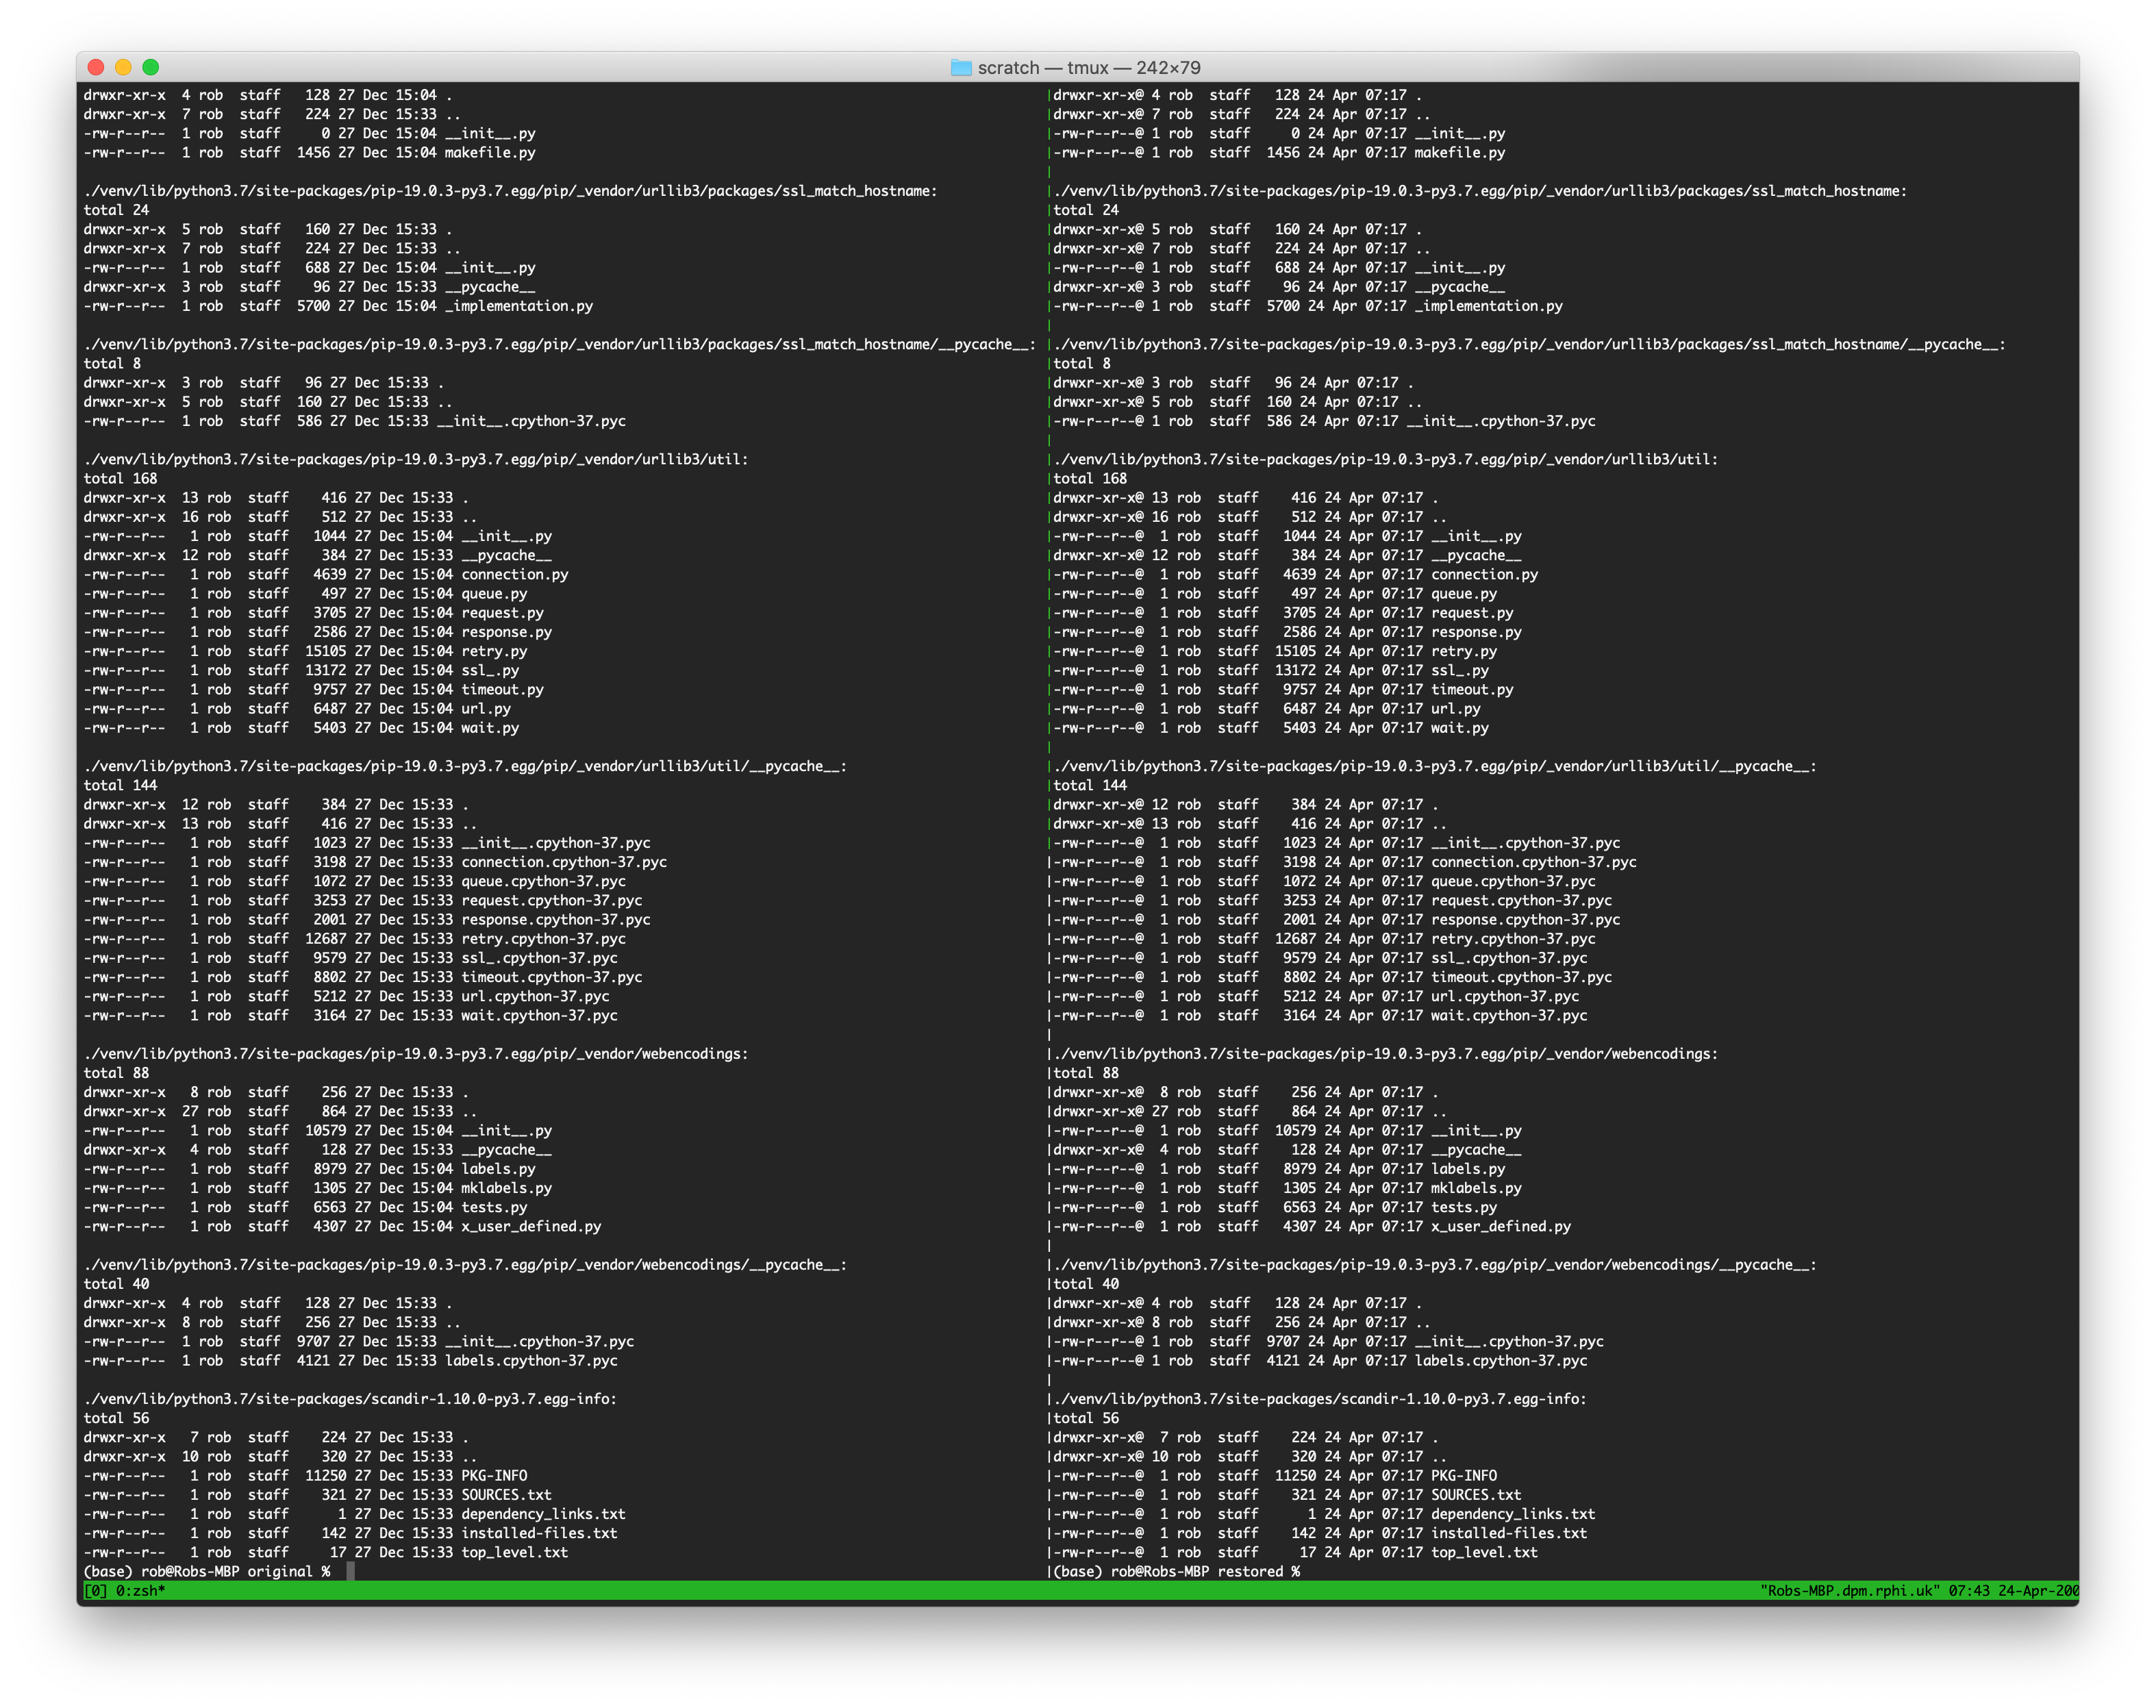
\includegraphics[width=1.1\linewidth]{img/screenshots/perms}
	\caption{Output of \texttt{ls -alR} for the original and restored versions of the test directory}
	\label{fig:perms}
\end{figure}

\begin{figure}
	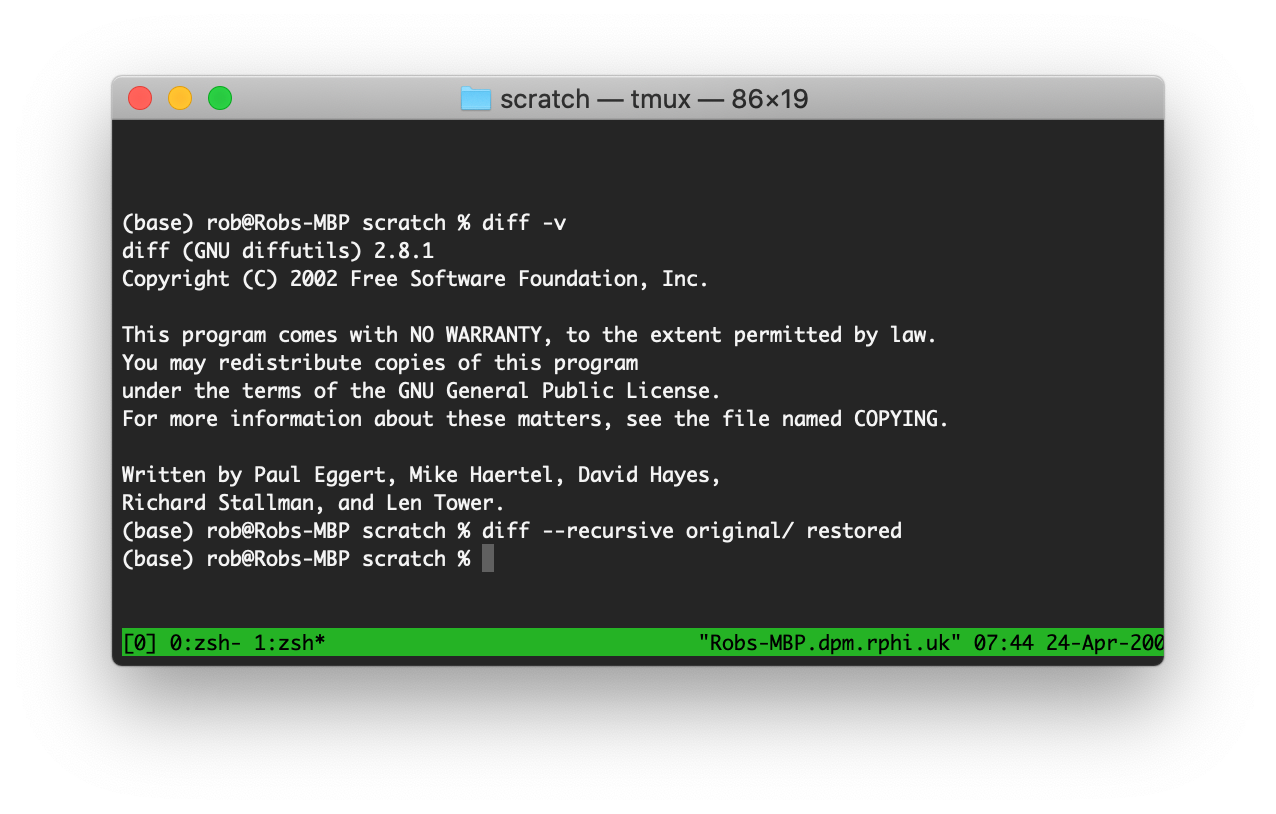
\includegraphics[width=0.9\linewidth]{img/screenshots/diff}
	\caption{Output of the \texttt{diff --recursive} command on the original and restored versions of the test directory}
	\label{fig:diff}
\end{figure}

% use the following and \cite{} as above if you use BibTeX
% otherwise generate bibtem entries
\bibliographystyle{IEEEtran}
\bibliography{costor-references.bib}

\end{document}
